
%% bare_jrnl.tex
%% V1.4b
%% 2015/08/26
%% by Michael Shell
%% see http://www.michaelshell.org/
%% for current contact information.
%%
%% This is a skeleton file demonstrating the use of IEEEtran.cls
%% (requires IEEEtran.cls version 1.8b or later) with an IEEE
%% journal paper.
%%
%% Support sites:
%% http://www.michaelshell.org/tex/ieeetran/
%% http://www.ctan.org/pkg/ieeetran
%% and
%% http://www.ieee.org/

%%*************************************************************************
%% Legal Notice:
%% This code is offered as-is without any warranty either expressed or
%% implied; without even the implied warranty of MERCHANTABILITY or
%% FITNESS FOR A PARTICULAR PURPOSE! 
%% User assumes all risk.
%% In no event shall the IEEE or any contributor to this code be liable for
%% any damages or losses, including, but not limited to, incidental,
%% consequential, or any other damages, resulting from the use or misuse
%% of any information contained here.
%%
%% All comments are the opinions of their respective authors and are not
%% necessarily endorsed by the IEEE.
%%
%% This work is distributed under the LaTeX Project Public License (LPPL)
%% ( http://www.latex-project.org/ ) version 1.3, and may be freely used,
%% distributed and modified. A copy of the LPPL, version 1.3, is included
%% in the base LaTeX documentation of all distributions of LaTeX released
%% 2003/12/01 or later.
%% Retain all contribution notices and credits.
%% ** Modified files should be clearly indicated as such, including  **
%% ** renaming them and changing author support contact information. **
%%*************************************************************************


% *** Authors should verify (and, if needed, correct) their LaTeX system  ***
% *** with the testflow diagnostic prior to trusting their LaTeX platform ***
% *** with production work. The IEEE's font choices and paper sizes can   ***
% *** trigger bugs that do not appear when using other class files.       ***                          ***
% The testflow support page is at:
% http://www.michaelshell.org/tex/testflow/



\documentclass[journal]{IEEEtran}
%
% If IEEEtran.cls has not been installed into the LaTeX system files,
% manually specify the path to it like:
% \documentclass[journal]{../sty/IEEEtran}
% toggle for showing comments
\newif\ifprintcomments
\printcommentstrue
\input tevc_style.sty


% Some very useful LaTeX packages include:
% (uncomment the ones you want to load)


% *** MISC UTILITY PACKAGES ***
%
%\usepackage{ifpdf}
% Heiko Oberdiek's ifpdf.sty is very useful if you need conditional
% compilation based on whether the output is pdf or dvi.
% usage:
% \ifpdf
%   % pdf code
% \else
%   % dvi code
% \fi
% The latest version of ifpdf.sty can be obtained from:
% http://www.ctan.org/pkg/ifpdf
% Also, note that IEEEtran.cls V1.7 and later provides a builtin
% \ifCLASSINFOpdf conditional that works the same way.
% When switching from latex to pdflatex and vice-versa, the compiler may
% have to be run twice to clear warning/error messages.






% *** CITATION PACKAGES ***
%
%\usepackage{cite}
% cite.sty was written by Donald Arseneau
% V1.6 and later of IEEEtran pre-defines the format of the cite.sty package
% \cite{} output to follow that of the IEEE. Loading the cite package will
% result in citation numbers being automatically sorted and properly
% "compressed/ranged". e.g., [1], [9], [2], [7], [5], [6] without using
% cite.sty will become [1], [2], [5]--[7], [9] using cite.sty. cite.sty's
% \cite will automatically add leading space, if needed. Use cite.sty's
% noadjust option (cite.sty V3.8 and later) if you want to turn this off
% such as if a citation ever needs to be enclosed in parenthesis.
% cite.sty is already installed on most LaTeX systems. Be sure and use
% version 5.0 (2009-03-20) and later if using hyperref.sty.
% The latest version can be obtained at:
% http://www.ctan.org/pkg/cite
% The documentation is contained in the cite.sty file itself.






% *** GRAPHICS RELATED PACKAGES ***
%
\ifCLASSINFOpdf
  % \usepackage[pdftex]{graphicx}
  % declare the path(s) where your graphic files are
  % \graphicspath{{../pdf/}{../jpeg/}}
  % and their extensions so you won't have to specify these with
  % every instance of \includegraphics
  % \DeclareGraphicsExtensions{.pdf,.jpeg,.png}
\else
  % or other class option (dvipsone, dvipdf, if not using dvips). graphicx
  % will default to the driver specified in the system graphics.cfg if no
  % driver is specified.
  % \usepackage[dvips]{graphicx}
  % declare the path(s) where your graphic files are
  % \graphicspath{{../eps/}}
  % and their extensions so you won't have to specify these with
  % every instance of \includegraphics
  % \DeclareGraphicsExtensions{.eps}
\fi
% graphicx was written by David Carlisle and Sebastian Rahtz. It is
% required if you want graphics, photos, etc. graphicx.sty is already
% installed on most LaTeX systems. The latest version and documentation
% can be obtained at: 
% http://www.ctan.org/pkg/graphicx
% Another good source of documentation is "Using Imported Graphics in
% LaTeX2e" by Keith Reckdahl which can be found at:
% http://www.ctan.org/pkg/epslatex
%
% latex, and pdflatex in dvi mode, support graphics in encapsulated
% postscript (.eps) format. pdflatex in pdf mode supports graphics
% in .pdf, .jpeg, .png and .mps (metapost) formats. Users should ensure
% that all non-photo figures use a vector format (.eps, .pdf, .mps) and
% not a bitmapped formats (.jpeg, .png). The IEEE frowns on bitmapped formats
% which can result in "jaggedy"/blurry rendering of lines and letters as
% well as large increases in file sizes.
%
% You can find documentation about the pdfTeX application at:
% http://www.tug.org/applications/pdftex





% *** MATH PACKAGES ***
%
%\usepackage{amsmath}
% A popular package from the American Mathematical Society that provides
% many useful and powerful commands for dealing with mathematics.
%
% Note that the amsmath package sets \interdisplaylinepenalty to 10000
% thus preventing page breaks from occurring within multiline equations. Use:
%\interdisplaylinepenalty=2500
% after loading amsmath to restore such page breaks as IEEEtran.cls normally
% does. amsmath.sty is already installed on most LaTeX systems. The latest
% version and documentation can be obtained at:
% http://www.ctan.org/pkg/amsmath





% *** SPECIALIZED LIST PACKAGES ***
%
%\usepackage{algorithmic}
% algorithmic.sty was written by Peter Williams and Rogerio Brito.
% This package provides an algorithmic environment fo describing algorithms.
% You can use the algorithmic environment in-text or within a figure
% environment to provide for a floating algorithm. Do NOT use the algorithm
% floating environment provided by algorithm.sty (by the same authors) or
% algorithm2e.sty (by Christophe Fiorio) as the IEEE does not use dedicated
% algorithm float types and packages that provide these will not provide
% correct IEEE style captions. The latest version and documentation of
% algorithmic.sty can be obtained at:
% http://www.ctan.org/pkg/algorithms
% Also of interest may be the (relatively newer and more customizable)
% algorithmicx.sty package by Szasz Janos:
% http://www.ctan.org/pkg/algorithmicx




% *** ALIGNMENT PACKAGES ***
%
%\usepackage{array}
% Frank Mittelbach's and David Carlisle's array.sty patches and improves
% the standard LaTeX2e array and tabular environments to provide better
% appearance and additional user controls. As the default LaTeX2e table
% generation code is lacking to the point of almost being broken with
% respect to the quality of the end results, all users are strongly
% advised to use an enhanced (at the very least that provided by array.sty)
% set of table tools. array.sty is already installed on most systems. The
% latest version and documentation can be obtained at:
% http://www.ctan.org/pkg/array


% IEEEtran contains the IEEEeqnarray family of commands that can be used to
% generate multiline equations as well as matrices, tables, etc., of high
% quality.




% *** SUBFIGURE PACKAGES ***
%\ifCLASSOPTIONcompsoc
%  \usepackage[caption=false,font=normalsize,labelfont=sf,textfont=sf]{subfig}
%\else
%  \usepackage[caption=false,font=footnotesize]{subfig}
%\fi
% subfig.sty, written by Steven Douglas Cochran, is the modern replacement
% for subfigure.sty, the latter of which is no longer maintained and is
% incompatible with some LaTeX packages including fixltx2e. However,
% subfig.sty requires and automatically loads Axel Sommerfeldt's caption.sty
% which will override IEEEtran.cls' handling of captions and this will result
% in non-IEEE style figure/table captions. To prevent this problem, be sure
% and invoke subfig.sty's "caption=false" package option (available since
% subfig.sty version 1.3, 2005/06/28) as this is will preserve IEEEtran.cls
% handling of captions.
% Note that the Computer Society format requires a larger sans serif font
% than the serif footnote size font used in traditional IEEE formatting
% and thus the need to invoke different subfig.sty package options depending
% on whether compsoc mode has been enabled.
%
% The latest version and documentation of subfig.sty can be obtained at:
% http://www.ctan.org/pkg/subfig




% *** FLOAT PACKAGES ***
%
%\usepackage{fixltx2e}
% fixltx2e, the successor to the earlier fix2col.sty, was written by
% Frank Mittelbach and David Carlisle. This package corrects a few problems
% in the LaTeX2e kernel, the most notable of which is that in current
% LaTeX2e releases, the ordering of single and double column floats is not
% guaranteed to be preserved. Thus, an unpatched LaTeX2e can allow a
% single column figure to be placed prior to an earlier double column
% figure.
% Be aware that LaTeX2e kernels dated 2015 and later have fixltx2e.sty's
% corrections already built into the system in which case a warning will
% be issued if an attempt is made to load fixltx2e.sty as it is no longer
% needed.
% The latest version and documentation can be found at:
% http://www.ctan.org/pkg/fixltx2e


%\usepackage{stfloats}
% stfloats.sty was written by Sigitas Tolusis. This package gives LaTeX2e
% the ability to do double column floats at the bottom of the page as well
% as the top. (e.g., "\begin{figure*}[!b]" is not normally possible in
% LaTeX2e). It also provides a command:
%\fnbelowfloat
% to enable the placement of footnotes below bottom floats (the standard
% LaTeX2e kernel puts them above bottom floats). This is an invasive package
% which rewrites many portions of the LaTeX2e float routines. It may not work
% with other packages that modify the LaTeX2e float routines. The latest
% version and documentation can be obtained at:
% http://www.ctan.org/pkg/stfloats
% Do not use the stfloats baselinefloat ability as the IEEE does not allow
% \baselineskip to stretch. Authors submitting work to the IEEE should note
% that the IEEE rarely uses double column equations and that authors should try
% to avoid such use. Do not be tempted to use the cuted.sty or midfloat.sty
% packages (also by Sigitas Tolusis) as the IEEE does not format its papers in
% such ways.
% Do not attempt to use stfloats with fixltx2e as they are incompatible.
% Instead, use Morten Hogholm'a dblfloatfix which combines the features
% of both fixltx2e and stfloats:
%
% \usepackage{dblfloatfix}
% The latest version can be found at:
% http://www.ctan.org/pkg/dblfloatfix




%\ifCLASSOPTIONcaptionsoff
%  \usepackage[nomarkers]{endfloat}
% \let\MYoriglatexcaption\caption
% \renewcommand{\caption}[2][\relax]{\MYoriglatexcaption[#2]{#2}}
%\fi
% endfloat.sty was written by James Darrell McCauley, Jeff Goldberg and 
% Axel Sommerfeldt. This package may be useful when used in conjunction with 
% IEEEtran.cls'  captionsoff option. Some IEEE journals/societies require that
% submissions have lists of figures/tables at the end of the paper and that
% figures/tables without any captions are placed on a page by themselves at
% the end of the document. If needed, the draftcls IEEEtran class option or
% \CLASSINPUTbaselinestretch interface can be used to increase the line
% spacing as well. Be sure and use the nomarkers option of endfloat to
% prevent endfloat from "marking" where the figures would have been placed
% in the text. The two hack lines of code above are a slight modification of
% that suggested by in the endfloat docs (section 8.4.1) to ensure that
% the full captions always appear in the list of figures/tables - even if
% the user used the short optional argument of \caption[]{}.
% IEEE papers do not typically make use of \caption[]'s optional argument,
% so this should not be an issue. A similar trick can be used to disable
% captions of packages such as subfig.sty that lack options to turn off
% the subcaptions:
% For subfig.sty:
% \let\MYorigsubfloat\subfloat
% \renewcommand{\subfloat}[2][\relax]{\MYorigsubfloat[]{#2}}
% However, the above trick will not work if both optional arguments of
% the \subfloat command are used. Furthermore, there needs to be a
% description of each subfigure *somewhere* and endfloat does not add
% subfigure captions to its list of figures. Thus, the best approach is to
% avoid the use of subfigure captions (many IEEE journals avoid them anyway)
% and instead reference/explain all the subfigures within the main caption.
% The latest version of endfloat.sty and its documentation can obtained at:
% http://www.ctan.org/pkg/endfloat
%
% The IEEEtran \ifCLASSOPTIONcaptionsoff conditional can also be used
% later in the document, say, to conditionally put the References on a 
% page by themselves.




% *** PDF, URL AND HYPERLINK PACKAGES ***
%
%\usepackage{url}
% url.sty was written by Donald Arseneau. It provides better support for
% handling and breaking URLs. url.sty is already installed on most LaTeX
% systems. The latest version and documentation can be obtained at:
% http://www.ctan.org/pkg/url
% Basically, \url{my_url_here}.




% *** Do not adjust lengths that control margins, column widths, etc. ***
% *** Do not use packages that alter fonts (such as pslatex).         ***
% There should be no need to do such things with IEEEtran.cls V1.6 and later.
% (Unless specifically asked to do so by the journal or conference you plan
% to submit to, of course. )


% correct bad hyphenation here
\hyphenation{op-tical net-works semi-conduc-tor}


\begin{document}
%
% paper title
% Titles are generally capitalized except for words such as a, an, and, as,
% at, but, by, for, in, nor, of, on, or, the, to and up, which are usually
% not capitalized unless they are the first or last word of the title.
% Linebreaks \\ can be used within to get better formatting as desired.
% Do not put math or special symbols in the title.
\title{An Iterative Two-stage Multi-fidelity Optimization Algorithm for Solving Computationally Expensive Problems}
%
%
% author names and IEEE memberships
% note positions of commas and nonbreaking spaces ( ~ ) LaTeX will not break
% a structure at a ~ so this keeps an author's name from being broken across
% two lines.
% use \thanks{} to gain access to the first footnote area
% a separate \thanks must be used for each paragraph as LaTeX2e's \thanks
% was not built to handle multiple paragraphs
%

% \author{Michael~Shell,~\IEEEmembership{Member,~IEEE,}
%         John~Doe,~\IEEEmembership{Fellow,~OSA,}
%         and~Jane~Doe,~\IEEEmembership{Life~Fellow,~IEEE}% <-this % stops a space
% \thanks{M. Shell was with the Department
% of Electrical and Computer Engineering, Georgia Institute of Technology, Atlanta,
% GA, 30332 USA e-mail: (see http://www.michaelshell.org/contact.html).}% <-this % stops a space
% \thanks{J. Doe and J. Doe are with Anonymous University.}% <-this % stops a space
% \thanks{Manuscript received April 19, 2005; revised August 26, 2015.}}

\author{Angus~Kenny,~Tapabrata~Ray,~and~Hemant~Kumar~Singh% <-this % stops a space
\thanks{The authors are with the School of Engineering and Information Technology, The University of New South Wales, Australia.\\Emails: \{angus.kenny, t.ray, h.singh\}@adfa.edu.au.}}
% of Electrical and Computer Engineering, Georgia Institute of Technology, Atlanta,
% GA, 30332 USA e-mail: (see http://www.michaelshell.org/contact.html).}% <-this % stops a space
% \thanks{J. Doe and J. Doe are with Anonymous University.}% <-this % stops a space
% \thanks{Manuscript received April 19, 2005; revised August 26, 2015.}}

% note the % following the last \IEEEmembership and also \thanks - 
% these prevent an unwanted space from occurring between the last author name
% and the end of the author line. i.e., if you had this:
% 
% \author{....lastname \thanks{...} \thanks{...} }
%                     ^------------^------------^----Do not want these spaces!
%
% a space would be appended to the last name and could cause every name on that
% line to be shifted left slightly. This is one of those "LaTeX things". For
% instance, "\textbf{A} \textbf{B}" will typeset as "A B" not "AB". To get
% "AB" then you have to do: "\textbf{A}\textbf{B}"
% \thanks is no different in this regard, so shield the last } of each \thanks
% that ends a line with a % and do not let a space in before the next \thanks.
% Spaces after \IEEEmembership other than the last one are OK (and needed) as
% you are supposed to have spaces between the names. For what it is worth,
% this is a minor point as most people would not even notice if the said evil
% space somehow managed to creep in.



% The paper headers
\markboth{Journal of \LaTeX\ Class Files,~Vol.~14, No.~8, August~2015}%
{Shell \MakeLowercase{\textit{et al.}}: Bare Demo of IEEEtran.cls for IEEE Journals}
% The only time the second header will appear is for the odd numbered pages
% after the title page when using the twoside option.
% 
% *** Note that you probably will NOT want to include the author's ***
% *** name in the headers of peer review papers.                   ***
% You can use \ifCLASSOPTIONpeerreview for conditional compilation here if
% you desire.




% If you want to put a publisher's ID mark on the page you can do it like
% this:
%\IEEEpubid{0000--0000/00\$00.00~\copyright~2015 IEEE}
% Remember, if you use this you must call \IEEEpubidadjcol in the second
% column for its text to clear the IEEEpubid mark.



% use for special paper notices
%\IEEEspecialpapernotice{(Invited Paper)}




% make the title area
\maketitle

% As a general rule, do not put math, special symbols or citations
% in the abstract or keywords.
\begin{abstract}
The abstract goes here.

\angus{Angus can make comments using \texttt{\textbackslash{}angus\{comment\}}}

\ray{Ray can make comments using \texttt{\textbackslash{}ray\{comment\}}}

\hemant{Hemant can make comments using \texttt{\textbackslash{}hemant\{comment\}}}
\end{abstract}

% Note that keywords are not normally used for peerreview papers.
\begin{IEEEkeywords}
IEEE, IEEEtran, journal, \LaTeX, paper, template.
\end{IEEEkeywords}






% For peer review papers, you can put extra information on the cover
% page as needed:
% \ifCLASSOPTIONpeerreview
% \begin{center} \bfseries EDICS Category: 3-BBND \end{center}
% \fi
%
% For peerreview papers, this IEEEtran command inserts a page break and
% creates the second title. It will be ignored for other modes.
\IEEEpeerreviewmaketitle



\section{Introduction}
% The very first letter is a 2 line initial drop letter followed
% by the rest of the first word in caps.
% 
% form to use if the first word consists of a single letter:
% \IEEEPARstart{A}{demo} file is ....
% 
% form to use if you need the single drop letter followed by
% normal text (unknown if ever used by the IEEE):
% \IEEEPARstart{A}{}demo file is ....
% 
% Some journals put the first two words in caps:
% \IEEEPARstart{T}{his demo} file is ....
% 
% Here we have the typical use of a "T" for an initial drop letter
% and "HIS" in caps to complete the first word.

% \hemant{IEEE requires use of US versions of the spelling ('-ize').}
\IEEEPARstart{M}{any} real-world engineering design problems require estimation of responses that are intractable for exact or analytical methods. In such cases, two alternatives are commonly resorted to: numerical simulations and physical testing of a prototype~\cite{forrester2008engineering}. When used in-loop during design optimization using iterative methods such as evolutionary algorithms~(EAs), both of these methods tend to be prohibitively slow; as well as potentially cost and resource intensive~\cite{jin2009systems}. Such optimization problems where each design evaluation incurs significant cost in any form are referred to as computationally expensive optimization problems.

Simulation-based optimization~(SO) refers to the methods that deal with optimization problems involving  numerical simulations\footnote{For brevity, the discussion is restricted to simulation-based design, but the same principles can be applied to other expensive optimization such as those involving physical prototyping.}. Typically, the these methods make use of surrogate approximations, also referred to as metamodels, to reduce the computational expense~\cite{amaran2016simulation}. The basic principle is to use historical information from previously evaluated designs to build a surrogate model of the response landscape. The predicted values from these surrogate models can be then utilized to determine new candidate solutions that are likely to be competent when evaluated using the true~(time consuming) simulation. Through this informed pre-selection, the number of expensive evaluations can be significantly reduced during the optimization. 

% A the production and testing of a prototype model can be probitively expensive, in terms of both time and cost. For these types of problem instances, numerical simulations --- such as finite element analysis (FEA) and computational fluid dynammics (CFD) --- can be employed to predict the outcome of various design choices. Simulation optimisation (SO) is an important tool which allows large design spaces to be searched, the merits of various candidate solutions to be approximated and inferences to be made about how those candidates might be improved --- all relatively cheaply.

% The principle behind SO is to iteratively use historical information from previous numerical simulations to construct a surrogate model (such as a kriging model) of the random field representing the fitness of a solution, with respect to its input variables. This model is searched using some optimisation technique, to find a new candidate --- or set of candidates --- which the model predicts will produce a good outcome when simulated. The data from this new simulation is incorporated into the surrogate model and the process continues.

% Although conducting a numerical simulation is not usually as expensive as producing and testing a physical prototype, it does incur a significant cost; with some complex FEA or CFD simulations taking several days to complete. Often, the allowed computational budget is given as a fixed amount, therefore it is important to ensure that this budget is used as efficiently as possible. In order to address this concern, the field of multi-fidelity simulation optimisation (MFSO) was developed.

Some numerical simulation processes allow control over the resolution, or fidelity, of the data they produce. For example, in finite element analysis~(FEA) or computational fluid dynamic~(CFD) simulations, the mesh size can be controlled to yield solutions with different fidelities~\cite{branke2016efficient}. A coarse mesh yields a low-fidelity~(LF) performance estimate that is relatively fast but less accurate, while a fine mesh yields a high-fidelity~(HF) estimate that is relatively more time consuming but more accurate. Multi-fidelity SO methods~(MFSO) are a special class of SO methods that attempt to efficiently combine the information from different fidelities with an eventual aim of searching for optimal HF designs. 

% 
% However, by combining information from both high- and low-fidelity simulations, MFSO methods can produce good quality approximations for a much lower computational cost.

% FEA simulations this can be controlled by the mesh density, and in CFD simulations it can be controlled by the number of iterations the simulation is run for. While these lower-fidelity simulations are cheaper to produce, there is a trade-off in the accuracy of their predictions.

% However, by combining information from both high- and low-fidelity simulations, MFSO methods can produce good quality approximations for a much lower computational cost.
% \hemant{Insert all the references.}
A number of different approaches to MFSO have been explored in the literature. Many of these approaches are based on the co-kriging technique described by Forrester et al.~\cite{forrester2007multi} which correlates the two sets of data, cheap and expensive, to produce a single prediction model. This technique is an extension of the autoregressive model first introduced by Kennedy and O'Hagan~\cite{kennedy2000predicting}. The two key aspects in which the different methods in this category deviate from each other, is in how they collect these data and also how they search the model for potential candidates. Laurenceau and Sagaut~\cite{laurenceau2008building} investigated a number of different sampling methods for use with kriging and co-kriging in an airfoil design problem. Perdikaris et al.~\cite{perdikaris2015multi} incorporate elements of statistical learning into a co-kriging framework to cross-correlate ensembles of multi-fidelity surrogate models. Yang et al.~\cite{yang2019physics} take a physics-informed approach, constructing models based on sparsely observed domain knowledge, representing unknowns as random variables or fields which are regressed using elements of co-kriging. Giraldo et al.~\cite{giraldo2020cokriging} provide an extension to co-kriging for use when the secondary variable is functional, based on the work of Goulard and Voltz~\cite{goulard1993geostatistical}.

Among the approaches that do not use co-kriging models, some of the prominent ones include the following. Lv et al.~\cite{lv2021multi} employ a canonical correlation analysis-based model, in which the least squares method is used to determine optimal parameters.  Ariyarit and Kanazaki~\cite{ariyarit2017multi} use a hybrid method which employs a kriging model to estimate local deviations and a radial basis function to approximate the global model in airfoil design problems. Hebbal et al.~\cite{hebbal2021multi} and Cutajar et al.~\cite{cutajar2019deep} both use machine learning techniques that treat the layers of a deep Gaussian process as different fidelity levels to capture non-linear correlations between fidelities. Xu et al.~\cite{xu2016mo2tos} use a two-stage process which first uses ordinal transformation to transform the original multi-dimensional design space into a one-dimensional ordinal space and then samples from this ordinal space using a method based on the optimal computational budget allocation (OCBA) algorithm proposed by Chen and Lee~\cite{chen2011stochastic}. Branke et al.~\cite{branke2016efficient} and Lim et al.~\cite{lim2008evolutionary} both take evolutionary approaches to solving MFSO problems.

Many of these approaches sample the low- and high-fidelity data \emph{a priori}, then build models based on these data and use some global search method to optimize them. To ensure these constructed models are properly representative, it is important to maintain a diversity of samples across the entire the design space; however, sampling without any prior knowledge can result in many computaional resources being expended in areas which do not contain any promising candidates. Of those which do sample the data iteratively, information is typically only shared in one direction between the two datasets. Low-fidelity data is sampled randomly, or using some indepenent process, and used to inform where the high-fidelity data should be sampled from; but no information is then shared in the reverse direction, to inform the low-fidelity sampling in the next iteration. Again, this can result in computational resources being consumed unnecessarily in regions of the search space which are unproductive, especially in high-dimensional problems. 

% \hemant{Elaborate why that may be problematic}. 

To overcome these limitations and improve the performance for MFSO, this paper proposes an iterative two-stage, bound-constrained, single-objective multi-fidelity optimisation problems, referred to here as \AlgName{}. It uses previously obtained information about promising areas of the search space to define a restricted neighbourhood using a guided differential evolution (DE) process on a kriging model of the low-fidelity data. This neighbourhood is then sampled from and searched, using a method derived from OCBA, to determine a set of candidates to undergo low-fidelity simulation. The information from these simulations is used to update the low-fidelity model and also a co-kriging-based surrogate model of the high-fidelity data, which is searched globally using DE to find a suitable candidate for high-fidelity simulation. Finally, these high-fidelity data is used to update the surrogate model and also to help determine the restricted neighbourhood in the next iteration. By using the high-fidelity simulation information to inform and restrict the region of interest while searching the low-fidelity model, \AlgName{} allows two-way information sharing between the sets of data. The performance of the \AlgName{} model is compared against a baseline co-kriging-based MFSO algorithm on two separate datasets. The first is a common set of multi-fidelity test-functions from the literature, and the second is a set of multi-fidelity test functions that are generated from standard test functions using the methods described in the paper by Wang et al. In addition to this, some important properties of \AlgName{} are also investigated.

The remainder of this paper is organized as follows. Section~\ref{sec:back} provides the fundamentals and background of the proposed model, along with a description of the type of problems tackled and related work. The \AlgName{} algorithm is detailed in Section~\ref{sec:method}, describing all of its constituent parts and detailing some similarities and differences with a related technique from the literature. Experimental design and datasets are discussed in Section~\ref{sec:exp}, with Section~\ref{sec:results} giving the results of these experiments and a discussion of their implications. Finally, Section~\ref{sec:conc} provides the conclusion and outlines any future directions of research.

% \hemant{I note that the discussion of existing works has been quite short. If the target is TEVC, a strategic decision is required at this point - whether we are going for a `Letter' (up to 9 pages) or a regular paper (up to 15 pages). If regular paper, then a more extensive  literature review section is required, discussing a much larger array of works and some trends in the approaches. If letter, then perhaps we can get away with short discussion as per current Section~I, but we should still provide a clear motivation by identifying the limitations of the previous approaches. For Section II, there needs to be a substantial reduction in the discussion of what's known to be standard. This includes, for example, the mathematical formulae with regards to Kriging/co-kriging formulation. The overall section in my opinion should not be more than 1 page (give or take)}. 


\section{Background and Related Work}\label{sec:back}
This section details the type of problem \AlgName{} is designed to address; provides information about two critical components that are used in its construction; and gives a brief summary of another method which is similar to \AlgName{} from the literature.

\subsection{Problem type}
The algorithm presented here is designed to address bound-constrained, single-objective, multi-fidelity optimisation problems with continuous variables. Here, the terms bound-constrained and continuous imply that a variable may have an upper- or lower-bound which it cannot exceed, but that it may take any value (precision issues notwithstanding) between these bounds in the decision space; and that there are no regions in the objective space which are forbidden. 

Let $P$ be a problem instance with $D$ decision variables and let $\V{x} \in \prod^D_{i=1}[l_i,u_i]$ be a \emph{solution} to $P$, represented by a real vector\footnote{Bold type is used here to indicate a vector (indexed by superscript) and regular type is used for elements (indexed by subscript). E.g., $\V{x}^i$ is the $i$th indexed vector, and $x_j^i$ is the $j$th element of the $i$th vector.} $\V{x}$ such that $l_i \le x_i \le u_i$ for all ${i \in [D]}$, where $\V{l},\V{u} \in \mathbb{R}^D$ are the lower- and upper-bounds, respectively\footnote{To conserve space, the following shorthand is used in this paper: ${[k] = \{1,2,\dots,k\}}$ and $[k^*] = \{0,1,\dots,k-1\}$.}. The \emph{objective value} of a solution to $P$ is given by the function
\begin{equation}
f:\displaystyle\prod^D_{i=1}[l_i,u_i]\to \mathbb{R},\ \V{x} \mapsto f(\V{x})\,, \label{eq:objective}
\end{equation}
which is typically smooth. When this objective value is minimized, the so-called \emph{optimal} solution to $P$ is $\V{x}^*$, such that $f(\V{x}^*) \leq f(\V{x})$ for all $\V{x} \in \prod^D_{i=1}[l_i,u_i]$, although it may be maximized without loss of generality.

Examples of these types of problems abound in the field of engineering design~\cite{deb2012optimization,forrester2008engineering} and often they require some form of numerical simulation to compute the objective value of their solutions. This numerical simulation can be very computationally expensive, therefore researchers often employ artificial test functions when developing algorithms. While not generally being an accurate model for the behaviour of real-world problems, test functions are very fast to evaluate and can be customized to gauge the performance of algorithms on a variety of fitness landscapes.

% One advantage of numerical simulation is that the fidelity of evaluated objective values can often be controlled, trading accuracy of the simulation for computational budget~\cite{branke2016efficient}. This effect is difficult to model using test functions as a low-fidelity function must still have some correlation to the true function in order to be useful, but also must contain enough noise to obfuscate its behaviour. The experiments detailed in Section~\ref{sec:exp} use datasets generated by two different methods from the literature.

The dataset in Lv et al.~\cite{lv2021multi} uses the customized addition, removal and modification of terms to produce a transformed function with a desired correlation to the original.
% For example, the pair of high- and low-fidelity functions
% \begin{align*}
% f_H(\V{x}) &= \displaystyle\sum^2_{i=1}\left(x_i^4 - 16x_i^2 + 5x_i\right)\,,\\ 
% f_L(\V{x}) &= 0.5\displaystyle\sum^2_{i=1}\left(x_i^4 - 16x_i^2\right)\,, 
% \end{align*}
% have a correlation coefficient of $0.79$ over $\V{x} \in [0,1]^2$. 
While this method allows control over the shape of the fitness landscape, it requires analysing each test function individually and only permits a single level of fidelity for each transformation.

The second strategy introduces external noise which models the errors that occur when simulation fidelity is decreased. Wang et al.~\cite{wang2017generic} analysed the behaviour of many numerical simulations under different fidelity conditions and 
% the following three types of errors:
% \begin{enumerate}
% \item \emph{Resolution errors:} The landscape of resolution errors is multimodal due to the inconsistency of global and local errors. It is deterministic but gets smoother when the fidelity level increases.
% \item \emph{Stochastic errors:} The errors are stochastic, i.e., the fitness value of the same solution varies in different simulation runs. The stochastic error decreases as the fidelity level increases.
% \item \emph{Instability errors:} Representing failed simulations. A failure happens at a certain probability, and the probability decreases as the fidelity level increases.
% \end{enumerate}
% From this, they 
formulated a generic transformation function to turn any test function $f$ of the form in Equation~\ref{eq:objective} into a low-fidelity version $\tilde f$:
\begin{equation}
\tilde f: \displaystyle\prod^D_{i=1}[l_i,u_i] \times [0,10000] \to \mathbb{R},\ (\V{x},\phi) \mapsto f(\V{x}) + e(\V{x},\phi)\,,\label{eq:error-fn}
\end{equation}
% \begin{equation*}
% \tilde f(x,\phi) = f(x) + e(x,\phi),
% \end{equation*}
where $\phi$ is the \emph{fidelity level}, with $\tilde f(\V{x},10000) = f(\V{x})$ and $\tilde f(\V{x},0)$ having the worst possible correlation to $f(\V{x})$. The \emph{error function}, $e(\V{x},\phi)$ --- which returns a single real value --- can be one of ten different functions, all of which are independent of $f(\V{x})$.

Because the error function is always independent of $f(\V{x})$, this method can be applied to any test function at all; and because $\phi$ is real-valued, many different fidelity levels can be modelled easily--- although some analysis must still be performed if specific correlation coefficients are required.

\subsection{Kriging and co-kriging}

Originally arising from geostatistical methods used for ore valuation in mining research --- but since being applied across a number of domains --- is the so-called \emph{kriging} method~\cite{forrester2008engineering}. Kriging is an interpolation technique that uses a limited set of sampled data to predict the objective value at a point that has not been sampled yet.

Let $P$ be a problem instance with $D$ decision variables and let $X = \{\V{x}^1,\V{x}^2,\dots,\V{x}^n\}$ be a set of $n$ sample points with observed objective values $\V{y} = \{y_1,y_2,\dots,y_n\}$, where $\V{x}^i \in \mathbb{R}^D$ for $i \in [n]$. A kriging model of these sample data is the Gaussian process 
\begin{equation}
Y(\V{x}) = f(\V{x}) + Z(\V{x}),\label{eq:krig}
\end{equation}
where, $f(\V{x})$ is a polynomial regression function based on the sample data $\V{y}$ and encapsulates the main variations in the data. The function $Z(\V{x})$ is a Gaussian process with mean $0$, which models the residual error. As the mean of $Z(\V{x})$ is 0, $f(\V{x})$ is the mean of $Y(\V{x})$. 

% The correlation matrix $\Psi$ of $Y(\V{x})$ is
% \begin{equation}
% \text{cor}[Y(\V{x}^i),Y(\V{x}^l)] = \exp\left(-\displaystyle\sum^D_{j=1}\theta_j\mid x_j^i-x_j^l \mid ^{p_j}\right),
% \end{equation}
% where $p_j$ is a smoothness parameter (typically $p_j \in [1,2]$) and $\theta_j$ determines how much influence decision variable $j$ has for a given sample point. Both $\V{p}$ and $\V{\theta}$ have size $D$ and are usually determined using maximum likelihood estimation (MLE). Given the set of sample points $X$ and this correlation matrix $\Psi$, the predicted value $Y(\V{x}')$ can be computed using Equation~\ref{eq:krig}, employing regression to find $f(\V{x}')$ and by interpolation on $\Psi$ to find $Z(\V{x}')$.

% \medskip

Low-fidelity data is typically much cheaper to produce than high-fidelity data, a fact which the \emph{co-kriging} technique exploits to great effect. Adapted from Kennedy and O'Hagan's autoregressive model~\cite{kennedy2000predicting}, co-kriging correlates multiple sets of data with different fidelities to produce a single model that approximates the high-fidelity data. The residual error for a sample point evaluated at a given fidelity is recursively modelled as a function of the error of the same point evaluated at the fidelity below it --- until some foundational model with lowest fidelity is reached. Because of this, the Markov property must be assumed, that given a sample point evaluated at some fidelity, no more information about that point can be gained by evaluating it at a lower fidelity.

Let $X_H = \{\V{x}_H^1,\V{x}_H^2,\dots,\V{x}_H^n\}$ be the set of $n$ high-fidelity sample points with observed objective values $\V{y}_H = \{y_{H(1)},y_{H(2)},\dots,y_{H(n)}\}$ and $X_L = \{\V{x}_L^1,\V{x}_L^2,\dots,\V{x}_L^m\}$ be the set of $m$ low-fidelity\footnote{Although only two fidelity levels are employed here, without loss of generality, the method can be extended to an arbitrary number of fidelities.} sample points with observed objective values $\V{y}_L = \{y_{L(1)},y_{L(2)},\dots,y_{L(m)}\}$. A kriging model $Y_L(\V{x})$ of the low-fidelity data is constructed according to Equation~\ref{eq:krig}. Using this, the high-fidelity model is
\begin{equation}
Y_H(\V{x}) = \rho(\V{x})\mu_L(\V{x}) + Z_d(\V{x}),
\end{equation} 
where $\rho(\V{x})$ is a scaling factor, determined as part of the MLE of the second model; $\mu_L(\V{x})$ is the mean of $Y_L(\V{x})$; and $Z_d(\V{x})$ is a Gaussian process which models the difference between $Y_H(\V{x})$ and $\rho(\V{x})\mu_L(\V{x})$.

An in-depth mathematical treatment of kriging, co-kriging and how to use these models to make predictions can be found in~\cite{forrester2008engineering,forrester2007multi,kennedy2001bayesian,kennedy2000predicting}.

\subsection{Optimal computing budget allocation}

Stochastic simulation is a noisy process, requiring multiple simulation replications in order to accurately approximate the true fitness value of a given design. 
% This estimation becomes more accurate with an increased volume of replications; however, performing more replications consumes finite computing resources. Therefore, in the interest of efficiency, it is best to concentrate efforts on simulating promising designs.

Assuming a normal distribution, the mean fitness value for a design, $\mu$, is unknown, but it can be estimated by its sample mean $\hat{\mu}$. 
Given a set of $k$ candidate designs and a finite computing budget $T$, the optimal computing budget allocation (OCBA)~\cite{chen2011stochastic} method aims to find an allocation such that ${N_1 + N_2 + \dots + N_k = T}$, where $N_i$ is the total replications allocated to design $i$, in order to select the best design, $b \in [k]$, such that $\hat{\mu}_b < \hat{\mu}_i$ for all $i \in [k]$.

The probability that design $b$ actually \emph{is} the the best design is called the probability of correct selection (PCS).
% \begin{equation}
% PCS = P\{\tilde\mu_b < \tilde\mu_i,i \neq b\},
% \end{equation}
% where $\tilde\mu_i \sim \mathcal{N}\left(\hat{\mu}_i,\frac{\sigma_i^2}{N_i}\right)$ is the posterior distribution of the unknown mean of design $i$, $\mu_i$.
The PCS can be estimated using Monte Carlo simulation, but this is time-consuming; therefore, the following problem is formulated in~\cite{chen2011stochastic} to compute the approximate probability of correct selection (APCS):
\begin{align}
\underset{N_1,\dots,N_k}{\text{maximize}}&\quad 1 - \displaystyle\sum^k_{i=1,i\neq b}P\{\tilde\mu_b < \tilde\mu_i\}\,,\nonumber\\
\text{such that}& \quad \displaystyle\sum^k_{i=1}N_i = T\,, \quad N_i \geq 0,
\end{align}

Based on the work in~\cite{chen2011stochastic}, the APCS is asymptotically maximized (as $T \to \infty$) when
\begin{align}
\dfrac{N_i}{N_j} &= \left(\dfrac{\sigma_i/\delta_{b,i}}{\sigma_j/\delta_{b,j}}\right)^2\,,\label{eq:apcs1}\\[0.2cm]
N_b &= \sigma_b \sqrt{\displaystyle\sum^k_{i=1,i\neq b}\dfrac{N_i^2}{\sigma_i^2}}\,,\label{eq:apcs2}
\end{align}
where $N_i$ is the total replications allocated to design $i$ and $\delta_{b,i} = \hat{\mu}_b - \hat{\mu}_i$, for all $i,j\in \{1,2,\dots,k\}$ with $i \neq j \neq b$.

The implications of Equations~\ref{eq:apcs1} and~\ref{eq:apcs2} are such that additional computing resources are not only allocated to those designs with a small sample mean, but also to potentially promising designs that have a high variance. A high variance indicates uncertainty in the prediction, which increased volume of replications will help to address.

Using the above results, Algorithm~\ref{alg:ocba} details an iterative process to select a design, based on maximising APCS.

\begin{algorithm}[h!] 
\caption{$OCBA$ procedure}
\label{alg:ocba}
\algsetup{linenosize=\footnotesize}
{\footnotesize
\begin{algorithmic}[1]
\REQUIRE{$k$, number of designs; $T$, computing budget; $\Delta$, replications per update; $n_0$, initial replications.}
\ENSURE{$b$, index of best design.}
\STATE{$b \ot \emptyset$} \COMMENT{Initialize $b$}
\STATE{$N_i \ot n_0\,,\ \forall i \in [k]$} \COMMENT{Count initial replications}
\STATE{$\V{S}^i \ot Sim(n_0)\,,\ \forall i \in [k]$} \COMMENT{Perform initial replications}
\WHILE{$\displaystyle\sum_{i \in [k]} N_i < T$}\label{while-loop}
  \STATE{$\V{N}' \ot \V{N}$} \COMMENT{Store old allocations}
  \STATE{$\V{\hat{\mu}},\V{\hat{\sigma}} \ot Stats(\V{S}),\ \forall i \in [k]$} \COMMENT{Compute sample statistics}
  \STATE{$b \ot \text{argmin}_i\ \hat{\mu}_i,\ \forall i \in [k]$} \COMMENT{Update $b$}
  \STATE{$\V{N} \ot Allocate(\V{\hat{\mu}},\V{\hat{\sigma}},\V{N},\Delta)$} \COMMENT{Allocate $\Delta$ replications}
  \STATE{$S_i \ot Sim(N_i-N_i'),\ \forall i \in [k]$} \COMMENT{Perform additional simulations}
\ENDWHILE
\end{algorithmic}
}
\end{algorithm}

In this algorithm, $Sim(n)$ is a function that returns the output of running the stochastic simulation $n$ times; $Stats(\V{S})$ computes the sample statistics for a set of simulation outputs; and $Allocate(\V{\hat{\mu}},\V{\hat{\sigma}},\V{N},\Delta)$ is a function that allocates $\Delta$ replications among the designs, in accordance with Equations~\ref{eq:apcs1} and~\ref{eq:apcs2}.

\subsection{$MO^2TOS$}
Optimal computing budget allocation (OCBA) operates on the assumption that each stochastic simulation being performed will have the same input parameters, and does not consider the case where the fitness of a solution may be evaluated with different fidelities. The multi-fidelity optimisation with ordinal transformation and optimal sampling ($MO^2TOS$)~\cite{xu2016mo2tos} framework is a two-stage algorithm that addresses this consideration, by combining ideas from OCBA with ordinal transformation~\cite{xu2014ordinal}.

Given a problem instance $P$ and a finite computing budget $T$, the $MO^2TOS$ algorithm takes advantage of the relatively low cost of low-fidelity evaluations to identify promising regions of the search space that can subsequently be exploited by iterative high-fidelity evaluations.

A large population of solutions are evaluated in low-fidelity and then ranked by their evaluated value. This ranked population is then partitioned into equal-sized groups. The reason for ranking the solutions before partitioning, is to increase the probability that solutions which share a group are proximate to each other in the transformed objective space, as opposed to the original design space. As a result, regardless of where solutions may be, it is more likely that solutions within a group will have a similar performance.

These partitioned groups are treated as de facto ``designs'' for the purposes of OCBA allocation; however, instead of multiple simulation replications being performed on the same design, the allocations will determine how many solutions are selected from a group for high-fidelity evaluation.

Initially, each group has $n_0$ solutions selected --- without replacement --- and evaluated in high-fidelity. These results are used to determine the sample statistics of the groups. Equations~\ref{eq:apcs1} and~\ref{eq:apcs2} are used to allocate a portion of the total budget, $\Delta$, to the set of groups. Solutions are selected from these groups in accordance with this allocation, and evaluated in high-fidelity. The sample statistics are computed once again and the process repeats, while the total budget consumed is less than $T$.

The value of $\Delta$ is typically quite small, as there may be significant bias between the low- and high-fidelity evaluated data. By keeping $\Delta$ small, it ensures that the sample statistics of the groups are updated more frequently, meaning that the allocations are based more on the statistics of each group, as opposed to their intial partitioning.

The $MO^2TOS$ framework has some limitations, due to the fact that it samples the low-fidelity data \emph{a priori} and the fact that is a two-step process that operates directly on the high- and low-fidelity functions, as opposed to an iterative one. By sampling the data once, without any prior information, the sampling must occur uniformly across the entire design space. This means that unnecessary computational budget is likely to be expended in areas which are not helpful to the search. Similarly, it is necessary to initially evaluate $n_0$ solutions with high-fidelity from each partitioned group, which can result in unnecessary expenditure of computational budget as well.

\section{\AlgName{} Algorithm}\label{sec:method}
The multi-fidelity optimisation algorithm proposed in this paper is an iterative two-stage process, which maintains two separate surrogate models that share information between them. The first surrogate is a kriging model of the low-fidelity data. This model is searched to find the best potential candidates, within a restricted region, to evaluate with low-fidelity. The information from this search is used to update the first model and a co-kriging model that combines both low- and high-fidelity data to approximate the high-fidelity objective function. This second model is globally searched to determine a suitable candidate for high-fidelity evaluation, and these data is used to update the co-kriging model and to determine the neighbourhood for the next search of the low-fidelity surrogate. Algorithm~\ref{alg:main-alg} gives a description of this process, and the functions within are defined in the following subsections.

\begin{algorithm}[h!]
\caption{\AlgName{} procedure}
\label{alg:main-alg}
\algsetup{linenosize=\footnotesize}
{\footnotesize 
\begin{algorithmic}[1]
\REQUIRE{$P$, problem data; $N_{L_{max}}$, max size of low-fidelity population; $N_{e_{max}}$, maximum number of evaluations; $\rho$, parameter set for LocalOCBA.}
\ENSURE{Best solution found $\V{x}^\beta$.}
\STATE{$X_v \ot LHS(P),\ \forall v \in \{L,H\}$} \COMMENT{Generate initial populations}
\STATE{$A_v,N_e \ot f_v(X_v,0),\ \forall v \in \{L,H\}$} \COMMENT{Evaluate initial populations}
\STATE{$\V{x}^\beta \ot \emptyset$} \COMMENT{Initialize $\V{x}^\beta$} 
\WHILE{$N_e < N_{e_{max}}$}
  \STATE{$M_L \ot Krige(A_L)$} \COMMENT{Update low-fidelity kriging model}
  \STATE{$M_C \ot CoKrige(A_L,A_H)$} \COMMENT{Update co-kriging model}
  \STATE{$\V{x} \ot GlobalSearch(M_C)$} \COMMENT{Globally search co-kriging model}
  \STATE{$\V{\alpha},N_e \ot f_H(\V{x},N_e)$} \COMMENT{Evaluate and update total cost}
  \STATE{$A_H \ot A_H \cup \{\V{\alpha}\}$} \COMMENT{Add $\V{\alpha}$ to high-fidelity archive}
  \STATE{$\V{x}^\beta \ot \min(f_H(\V{x}^\beta),f_H(\V{x}))$} \COMMENT{Update best solution}
  \STATE{$\epsilon \ot Sigmoid(N_e,N_{e_{max}})$} \COMMENT{Determine size of neighbourhood}
  \STATE{$A_L,N_e \ot LocalOCBA(\rho,M_L,A_L,\V{x}^\beta,\epsilon)$} \COMMENT{Locally search low-fidelity model}
  \IF{$|A_L| > N_{L_{max}}$}
    \STATE{$A_L \ot Winnow(A_L,N_{L_{max}})$} \COMMENT{Control population size}
  \ENDIF
\ENDWHILE
\end{algorithmic}
}
\end{algorithm}

\subsection{Initialisation, evaluation and surrogate models}
The function $LHS(P)$ returns an initial population sampled from a latin hypercube with size $6D$ for high-fidelity and $18D$ for low-fidelity, where $D$ is the number of decision variables defined in the problem data $P$. The bounds of the hypercube are also defined in $P$. Latin hypercube sampling is used in order to start with as broad a picture of the search space as possible. Solutions are evaluated using the function $f_v(X,N_e)$, at some fidelity $v\in \{L,H\}$, which returns a set of ``archive'' pairs comprising the solution and its objective value. It also updates the total cost incurred, $N_e$. 

Two surrogate models are used, $Krige(A_L)$ takes the low-fidelity data and returns a kriging model approximating it, and $CoKrige(A_L,A_H)$ takes both the low- and high-fidelity archive data and returns a co-kriging model that approximates the fitness landscape of the high-fidelity data. The function $GlobalSearch(M_C)$ takes the co-kriging model as input and returns the best solution that can be found using some global search method. This output solution is evaluated in high-fidelity, the information from which is used to update the co-kriging model, and also to determine the restricted neighbourhood used to locally search the low-fidelity kriging model.

\subsection{Restricted neighbourhood}\label{subsec:restrict}
The correlation between the low- and high-fidelity data can vary wildly between problems, meaning identifying a promising region in the low-fidelity kriging model does not necessarily mean identifying a promising region in the high-fidelity co-kriging model. Therefore, instead of searching the low-fidelity model globally, it makes sense to search for promising candidates within a restricted neighbourhood, defined using information from the high-fidelity model. As the goal of performing low-fidelity evaluations in co-kriging models is to gain information about the shape of the fitness landscape, more than it is to find the ``best'' low-fidelity solution, restricting the neighbourhood in this way allows the algorithm to focus on the region of interest --- without getting ``distracted'' by global optima that might not be useful in the over-all search.

In order to restrict the region of interest, a so-called \emph{guided~DE} process is employed. In differential evolution (DE), assuming complete recombination occurs, a candidate child solution $x_c$ is produced from three parent solutions $\V{x}^1$, $\V{x}^2$ and $\V{x}^3$ with the following formula:
\begin{equation}
\V{x}^c = \V{x}^1 + F(\V{x}^2 - \V{x}^3)\,,
\end{equation}
with $F$ being a constant called the mutation factor. This is simply scaled vector addition, therefore this produced child $\V{x}^c$ can be ``nudged'' further towards a reference point (in this case $x_\beta$) by a similar process:
\begin{equation}\label{eq:nudge}
\V{x}^{c'} = \V{x}^c + \V{g}(\V{x}^\beta - \V{x}^c)\,,
\end{equation}
where $\V{G}$ is the so-called \emph{guide factor}. This is illustrated in Figure~\ref{fig:guide-DE}.

\begin{figure}[h!]
\centering
\adjustbox{max width=0.5\textwidth}{%
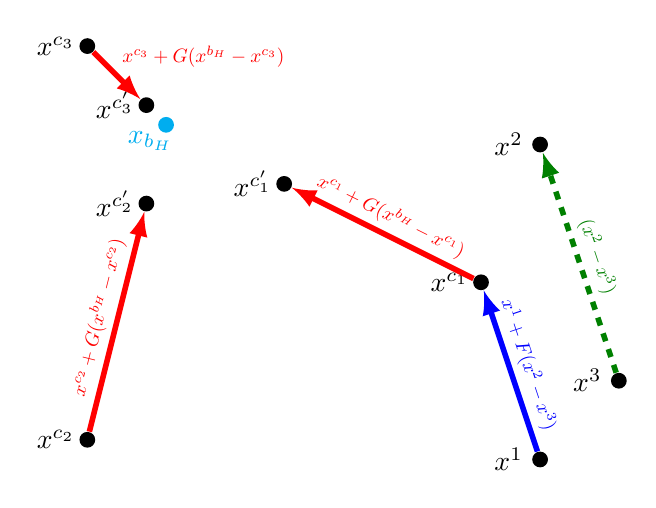
\begin{tikzpicture}

\node [fill, circle,inner sep=0pt,minimum size=2mm] (x1) at (0,0) {};
\node [fill, circle,inner sep=0pt,minimum size=2mm] (x3) at (1,1) {};
\node [fill, circle,inner sep=0pt,minimum size=2mm] (x2) at (0,4) {};
\node [fill, circle,inner sep=0pt,minimum size=2mm] (xc1) at (-0.75,2.25) {};
\node [fill, circle,inner sep=0pt,minimum size=2mm,color=cyan] (xb) at (-4.75,4.25) {};
\node [fill, circle,inner sep=0pt,minimum size=2mm] (xc1p) at (-3.25,3.5) {};
\node [fill, circle,inner sep=0pt,minimum size=2mm] (xc2) at (-5.75,0.25) {};
\node [fill, circle,inner sep=0pt,minimum size=2mm] (xc2p) at (-5,3.25) {};
\node [fill, circle,inner sep=0pt,minimum size=2mm] (xc3) at (-5.75,5.25) {};
\node [fill, circle,inner sep=0pt,minimum size=2mm] (xc3p) at (-5,4.5) {};

\node [xshift = -4mm] (x1t) at (x1) {$\V{x}^1$};
\node [xshift = -4mm] (x2t) at (x2) {$\V{x}^2$};
\node [xshift = -4mm] (x3t) at (x3) {$\V{x}^3$};
\node [xshift = -4mm] (xc1t) at (xc1) {$\V{x}^{c_1}$};
\node [xshift = -4mm] (xc2t) at (xc2) {$\V{x}^{c_2}$};
\node [xshift = -4mm] (xc3t) at (xc3) {$\V{x}^{c_3}$};
\node [xshift = -2mm,yshift = -2mm,color=cyan] (xbt) at (xb) {$x_{b_H}$};
\node [xshift = -4mm] (xc1pt) at (xc1p) {$\V{x}^{c_1'}$};
\node [xshift = -4mm] (xc2pt) at (xc2p) {$\V{x}^{c_2'}$};
\node [xshift = -4mm] (xc3pt) at (xc3p) {$\V{x}^{c_3'}$};

\draw [-latex,line width=2,color=Green,dashed] (x3) -- node[sloped,above,scale=0.7] {$(\V{x}^2-\V{x}^3)$} (x2);
\draw [-latex,line width=2,color=Blue] (x1) -- node[sloped,above,scale=0.7] {$\V{x}^1+F(\V{x}^2-\V{x}^3)$} (xc1);
\draw [-latex,line width=2,color=Red] (xc1) -- node[sloped,above,scale=0.7] {$\V{x}^{c_1}+G(\V{x}^{b_H}-\V{x}^{c_1})$} (xc1p);
\draw [-latex,line width=2,color=Red] (xc2) -- node[sloped,above,scale=0.7] {$\V{x}^{c_2}+G(\V{x}^{b_H}-\V{x}^{c_2})$} (xc2p);
\draw [-latex,line width=2,color=Red] (xc3) -- node[xshift=11mm,above,scale=0.7] {$\V{x}^{c_3}+G(\V{x}^{b_H}-\V{x}^{c_3})$} (xc3p);

\end{tikzpicture}
}
\caption{The DE recombination process can be ``guided'' towards the best high-fidelity solution found so far.}\label{fig:guide-DE}
\end{figure}

In this figure, it can be seen that $\V{x}^{c_1}$ is produced using $\V{x}^1$, $\V{x}^2$ and $\V{x}^3$, and then translated using Equation~\ref{eq:nudge} to produce $\V{x}^{c_1'}$. Child solutions $\V{x}^{c_2}$ and $\V{x}^{c_3}$ are produced using two other sets of solutions that are not pictured, and then translated using the same equation. If this process is continued, the result is a ``cloud'' of candidate solutions in the vicinity of $\V{x}^\beta$, the centre of the region of interest.

The guide factor determines how far the resulting solution is translated in the direction of $\V{x}^\beta$. At the beginning of the search, $\V{x}^\beta$ is determined by optimising a very coarse model built with sparse information, and cannot be trusted to be indicative of a promising region of the search space; as the search continues, the model becomes more accurate and the information it produces more trustworthy. Therefore, the algorithm should be explorative in the beginning of the search, but exploitative towards the end. One function which exhibits these properties is the logistic sigmoid curve
\begin{equation}
\epsilon = \dfrac{L}{1+e^{-k(x-x_0)}}\,,
\end{equation}
where $x_0$ is the $x$ value of the sigmoid's midpoint, $L$ is the curve's maximum and $k$ is the steepness parameter, which controls how fast the function ``ramps up''. The function $Sigmoid(N_e,N_{e_{max}})$ uses the total cost and maximum cost to compute this $\epsilon$ value. Figure~\ref{fig:logistic} gives a plot of the logistic sigmoid curve with $L=0.99$, $k=10$ and $x_0 = 0.2$. 
\begin{figure}[h!]
  \centering
  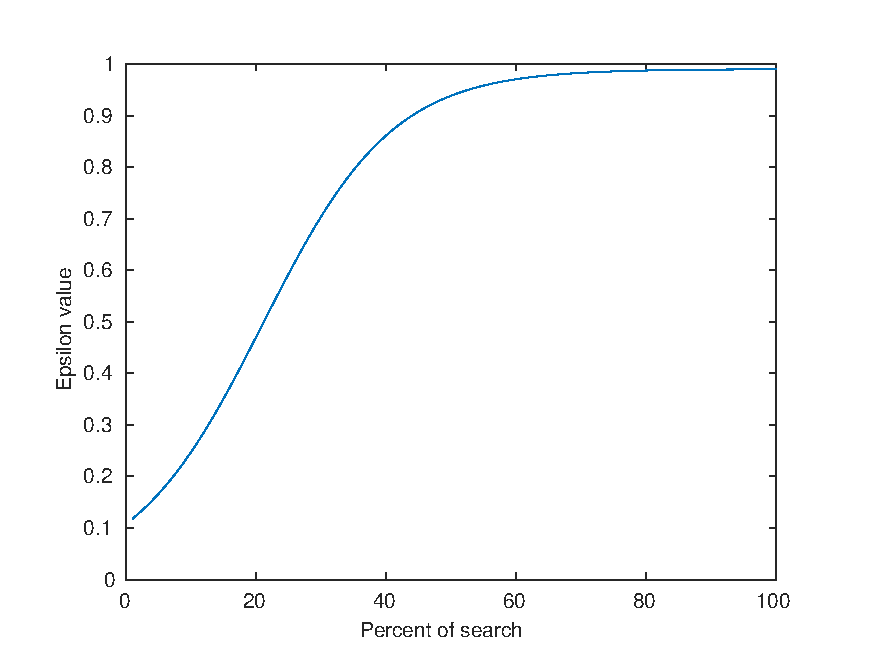
\includegraphics[width = 0.40\textwidth]{img/logistic.eps} 
  \caption{The logistic sigmoid curve flattens at around 80\%.} 
    \label{fig:logistic}
\end{figure}
Using this value, $\V{g}$ can be computed as:
\begin{equation}
\V{g} = \epsilon + (1-\epsilon)\V{r}\,,
\end{equation}
where $\V{r} \in [0,1]^D$ is a random vector with $D$ components, making $\V{g} \in [\epsilon,1]^D$ also a random vector. This ensures the cloud of candidate solutions around $\V{x}^\beta$ is sparse at the beginning of the search, allowing for better global exploration, while focusing the search more tightly on promising regions towards the end --- crucially, without adding any extra parameters. 

\subsection{LocalOCBA}\label{subsec:local}
Once the candidate solutions have been been generated in the vicinity of $\V{x}^\beta$, they must be selected from. As already stated, the goal of evaluating solutions in low-fidelity is not to optimize the low-fidelity objective function, but to provide as much information for the model as possible. The optimal computing budget allocation (OCBA) algorithm selects from a set of solutions with the goal of reducing uncertainty within simulation models (by allocating computing resources). This principle can be applied here, with some modifications, as described in Algorithm~\ref{alg:local-ocba}.

\begin{algorithm}[h!] 
\caption{$LocalOCBA$ procedure}
\label{alg:local-ocba}
\algsetup{linenosize=\footnotesize}
{\footnotesize
\begin{algorithmic}[1]
\REQUIRE{$\rho=\{\Delta_1$, total to be sampled; $\Delta_2$, samples per statistics update$\}$; $M$, low-fidelity model; $A_L$, low-fidelity archive; $\V{x}^\beta$, best high-fidelity solution ; $\epsilon$, sigmoid value; $N_e$, total cost incurred.}
\ENSURE{$A_L$, updated low-fidelity archive; $N_e$, updated total cost.}
\STATE{$X \ot GuidedDE(A_L,\V{x}^\beta,\epsilon)$} \COMMENT{Generate child population}
\STATE{$A_X \ot f_{M}(X)$} \COMMENT{Approximate each child by model $M$}
\STATE{$G,k \ot Partition(A_X)$} \COMMENT{Partition solutions}
\STATE{$S_i \ot \emptyset,\ \forall i \in [k]$} \COMMENT{Empty groups for selected solutions}
\WHILE{$\displaystyle\sum_{i \in [k]} |S_i| < \Delta_1$}\label{while-loop}
  \STATE{$\hat{\mu}_i,\hat{\sigma}_i \ot$ sample statistics for $S_i$, $\forall i \in [k]$ (if $|S_i| < 2$, use $G_i$)}
  \STATE{$R \ot GetRatios(\V{\hat{\mu}},\V{\hat{\sigma}})$} \COMMENT{compute allocation ratios}
  \STATE{$D \ot Allocate(R,S,G) : \displaystyle\sum_{i \in [k]}|D_i| = \Delta_2$} \COMMENT{Allocate $\Delta_2$ solutions according to ratios $R$}
  \STATE{$D_i,N_e \ot f_L(D_i,N_e),\ \forall i \in [k]$} \COMMENT{Evaluate allocated solutions}
  \STATE{$S_i \ot S_i \cup D_i,\ \forall i \in [k]$} \COMMENT{Add to selected solutions}
  \STATE{$G_i \ot G_i \setminus D_i,\ \forall i \in [k]$} \COMMENT{Selection without replacement}
\ENDWHILE
\STATE{$A_L \ot A_L \cup \displaystyle\bigcup_{i \in [k]} S_i$} \COMMENT{Combine all selected solutions}
\end{algorithmic}
}
\end{algorithm}

Here, the $GuidedDE(A_L,\V{x}^\beta,\epsilon)$ process is used to generate a set of candidate solutions, which are approximated using $f_M(X)$. This function takes a set of solutions and returns a set of pairs comprising the solution and its approximation on some model $M$. The solutions are ranked and partitioned using a clustering algorithm, based on their approximated value. The purpose of ranking the solutions first is to increase the probability that solutions within a clustered group will tend to have a similar performance to each other, regardless of their proximity in the decision space. This helps to ensure a diversity of solutions will be selected, while still preferencing the more promising candidates. The function $Partition(X)$ returns a set of solution groups $G$ and the number of groups $k$.

OCBA principles are used to select --- without replacement --- from these groups to populate a set of empty groups $S$. First, sample statistics are computed for all groups of selected solutions in $S$. If there are fewer than two solutions in a group, then its corresponding group in $G$ is used. The function $GetRatios(\V{\hat{\mu}},\V{\hat{\sigma}})$ uses these statistics to compute allocation ratios in accordance for each group with standard OCBA practice. These ratios are used by $Allocate(R,S,G)$ to allocate $\Delta_2$ solutions to be evaluated as low-fidelity and added to the selected solutions $S$.

Once $\Delta_1$ solutions have been selected, they are added to the low-fidelity archive, and the updated archive is returned.

\subsection{Population size control}
Due to the fact that many more low-fidelity solutions are added to the archive between each high-fidelity evaluation, the size of the low-fidelity archive can become too big for some kriging and co-kriging algorithms, or too concentrated if the search is focused on the same area for too long. Therefore, a maximum population size $N_{L_{max}}$ should be set such that once it reaches that threshold, the population should be maintained at that level. Choosing a steady-state method such as ranking the solutions by their value and selecting the top $N_{L_{max}}$ will cause the population to converge and lose diversity over time. As the purpose of maintaining the low-fidelity population is to provide the co-kriging model with information about the shape of the fitness landscape, this loss of diversity can be very detrimental. 

The function $Winnow(A_L,N_{L_{max}})$ takes an archive and a maximum size and returns a winnowed archive with exactly $N_{L_{max}}$ solutions. It does this by partitioning the solutions --- in the decision space --- into $N_{L_{max}}$ different groups using a clustering algorithm, such as $k$-means clustering. Most of these clusters will contain only one solution which is added to the winnowed archive; for those that have more than one solution, only the solution with the best value is selected. This ensures that the archive never has more than $N_{L_{max}}$ solutions, but diversity is maintained throughout the population.

\subsection{Similarities and differences to $MO^2TOS$}
There exist some similarities between \AlgName{} and the $MO^2TOS$ framework. For example, both use a two-step process of ordering a population of solutions and then selecting from them using ideas from OCBA. Despite the similarities, there are several key aspects which differentiate the two algorithms from each other. 

The biggest difference is that \AlgName{} is an iterative process, whereas $MO^2TOS$ is a two-step algorithm which is only run through one time. As $MO^2TOS$ only performs a single iteration, it cannot use any prior knowledge to determine where it should concentrate its resources when evaluating the initial low-fidelity population. Therefore, it must evaluate uniformly across the whole search space, and subsequently expend computational budget in areas which are not beneficial to the search. In contrast, \AlgName{} uses information from previous iterations, to identify promising areas of the search space that it can exploit.

Another difference is that $MO^2TOS$ operates on the high- and low-fidelity objective functions directly, across the entire search space. Solutions are selected using information from low-fidelity evaluations, to be evaluated in high-fidelity. \AlgName{} uses its ranking and selection phases in order to select from a neighbourhood of solutions that have been identified in a promising region of the search space. These selections are informed by a kriging model of the low-fidelity function, and selected for low-fidelity evaluation. The high-fidelity evaluations are determined by a separate search that is perfomed on the co-kriging model, updated by the selected low-fidelity evaluations. Because of this, it is not necessary to perform the initial $n_0$ evaluations before computing the sample statistics, as the goal is not to optimize the low-fidelity objective function, just select from a set of ranked candidates.

Finally, $MO^2TOS$ partitions the ranked population into equal-sized groups, whereas \AlgName{} uses a clustering algorithm to determine the number and size of partitions. This ensures that the average distance between groups in objective space is maximized.

\section{Numerical Experiments}\label{sec:exp}
The experiments were carried out on \angus{insert details of machine and OS here}. All code was implemented and executed in MATLAB\angus{version number}, with kriging and co-kriging models constructed using the ooDACE toolbox~\cite{oodace}.

The \AlgName{} algorithm was compared against a baseline co-kriging algorithm. Both algorithms were run 30 times on each problem instance for the equivalent of 2000 low-fidelity evaluations, recording the best objective value, the mean and standard deviation of the resulting solutions produced by each run.


\subsection{Datasets}
The experiments were run on a collection of bound-constrained, single-objective, multi-fidelity test functions that can be divided into two different datasets. The first set is a selection of problem instances taken from Lv~et~al.~\cite{lv2021multi}. Problems $f10$ to $f17$ were chosen from this dataset as they contain between three and eight decision variables, determined as a representative range of easy to difficult problems. The problem instances here are provided with explicit definitions for both the high- and low-fidelity functions.

The second set of problem instances is generated using the Griewank and Michalewicz test problems (Figures~\ref{fig:grie} and~\ref{fig:michal}), taken from the Virtual Library of Simulation Experiments~\cite{get-citation}. Each problem was instantiated with versions for three, five and eight decision variables. This matches the range of the first dataset, and also allows the performance of the algorithms to be judged across different sized problems in a more controlled environment. These test problems are not naturally multi-fidelity optimisation problems, so low-fidelity evaluations must be made by applying the methods described in~\cite{wang2017generic}. Two different error functions were tested for each instance, modelling two types of fidelity error: resolution and stochastic. An appropriate fidelity level $\phi$ for each problem was chosen by computing the square of the Pearson correlation coefficient $r^2$ for different fidelity values and selecting a value for $\phi$ such that $r^2$ was between 0.65 and 0.85, to be commensurate with the first dataset.

See Tables~\ref{tab:funcs} and~\ref{tab:errfuncs} in Appendix~\ref{app:testfuncs} for test function and error function equations, respectively.

\begin{figure}[h!]
  \centering
  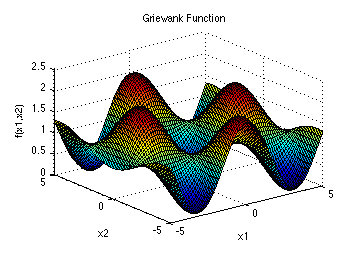
\includegraphics[width = 0.40\textwidth]{img/griewank.png} 
  \caption{The Griewank test function in 2D.\angus{will do a better version}} 
    \label{fig:grie}
\end{figure}
\begin{figure}[h!]
  \centering
  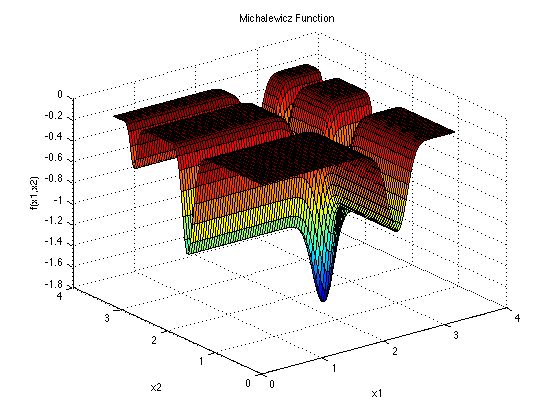
\includegraphics[width = 0.40\textwidth]{img/michal.png} 
  \caption{The Michalewicz test function in 2D.\angus{will do a better version}} 
    \label{fig:michal}
\end{figure}

\subsection{Baseline co-kriging algorithm}
Co-kriging is a popular approach to solving many multi-fidelity problems. The outer-loop of the \AlgName{} algorithm functions by iteratively updating a co-kriging model using data from a modified version of the OCBA procedure. In order to demonstrate the effectiveness of this new technique, the performance of \AlgName{} is compared against the baseline simple co-kriging algorithm given in Algorithm~\ref{alg:co-kriging}.

\begin{algorithm}[h!] 
\caption{Baseline co-kriging procedure}
\label{alg:co-kriging}
\algsetup{linenosize=\footnotesize}
{\footnotesize
\begin{algorithmic}[1]
\REQUIRE{$P$, problem data; $N_{L_{max}}$, max size of LF pop; $N_{e_{max}}$, maximum number of evaluations; $\Delta$, new LF per iteration.}
\ENSURE{Best solution found $\V{x}^\beta$.}
\STATE{$X_v \ot LHS(P),\ \forall v \in \{L,H\}$} \COMMENT{Generate initial populations}
\STATE{$\V{x}^\beta \ot \emptyset$} \COMMENT{Initialize $x_\beta$} 
\WHILE{$N_e < N_{e_{max}}$}
  \STATE{$A_L \ot A_L \cup LHS(\Delta)$} \COMMENT{Add $\Delta$ new solutions to LF archive}
  \IF{$|A_L| > N_{L_{max}}$}
    \STATE{$A_L \ot winnow(A_L,N_{L_{max}})$} \COMMENT{Control population size}
  \ENDIF
  \STATE{$M_C \ot CoKrige(A_L,A_H)$} \COMMENT{Update co-kriging model}
  \STATE{$\V{x} \ot GlobalSearch(M_C)$} \COMMENT{Globally search co-kriging model}
  \STATE{$\V{\alpha},N_e \ot f_H(\V{x},N_e)$} \COMMENT{Evaluate and update total cost}
  \STATE{$A_H \ot A_H \cup \{\V{\alpha}\}$} \COMMENT{Add $\V{\alpha}$ to high-fidelity archive}
  \STATE{$\V{x}^\beta \ot \min(f_H(\V{x}^\beta),f_H(\V{x}))$} \COMMENT{Update best solution}
\ENDWHILE
\end{algorithmic}
}
\end{algorithm}

The functions here have the same definitions as in Algorithm~\ref{alg:main-alg}. This procedure iteratively updates a co-kriging model by randomly sampling the low-fidelity data using a latin hypercube sampling (LHS) technique; however, the global search method remains the same.

\subsection{Parameters}
\AlgName{} can be viewed as a general framework into which various search and modeling methods can be ``plugged''. Therefore, its components can be divided into two categories: \AlgName{} specific components, which are intrinsic to its operation and whose parameters are also intrinsic; and, generic method components, such as global search techniques and modelling methods which can be substituted for other similar techniques, which come with their own parameters. The \AlgName{} specific parameters are discussed in Section~\ref{sec:method}; this section will detail the parameters for the generic search method used.

Differential evolution (DE) was used to globally search the updated co-kriging model. This DE was run over 30 generations with a crossover rate of 0.9, a mutation factor of 0.5 and a population size of 100.

The kriging models used are from the ooDACE toolbox~\cite{oodace}, with the default paramters.

\section{Results and Discussion}\label{sec:results}
\begin{table*}[h!]
\centering
\caption{Results on problems $f10$-$f17$ comparing the base-line co-kriging algorithm to \AlgName{}. Given are the number of decision variables ($D$), the square of the Pearson correlation coefficient ($r^2$), the best objective obtained, the mean best objective over the full set of runs ($\mu$) and the corresponding standard deviation ($\sigma$).}\label{tab:results}
% \begin{adjustbox}{width=\columnwidth}
\begin{tabular}{lrrrrrrrr} \toprule
& & & \multicolumn{3}{c}{Co-kriging} & \multicolumn{3}{c}{\AlgName{}}\\
\cmidrule(lr){4-6} \cmidrule(lr){7-9}
Instance & $D$ & $r^2$ &\multicolumn{1}{c}{best}&\multicolumn{1}{c}{\(\mu\)} & \multicolumn{1}{c}{\(\sigma\)}&\multicolumn{1}{c}{best}& \multicolumn{1}{c}{\(\mu\)}&\multicolumn{1}{c}{\(\sigma\)}\\ \midrule
%
$f10$ & 3 & 0.64 &        0 &  2.2960  &  3.5445  &       0 &   3.9189 &  5.3296\\
$f11$ & 3 & 0.74 &   0.0001 &  0.0110  &  0.0077  &  0.0004 &   0.0098 &  0.0064\\
$f12$ & 4 & 0.79 &  -9.5783 & -5.8853  &  1.5123  & -8.1107 &  -3.8007 &  1.3426\\
$f13$ & 4 & 0.89 &   0.6290 &  4.9366  &  5.0965  &  0.0519 &   0.3457 &  0.1971\\
$f14$ & 5 & 0.75 &   0.2509 &  0.2583  &  0.0039  &  0.2522 &   0.2607 &  0.0037\\
$f15$ & 6 & 0.78 & 104.2304 &  1700.28 &  2015.04 & 24.6278 & 152.9817 &144.6451\\
$f16$ & 8 & 0.82 & 7.3904   &  196.810 &  171.7771&  7.9240 &  75.2898 & 59.3423\\
$f17$ & 8 & 0.79 & -2.5859  &  42.0074 &  153.4414& -3.0161 & -2.8355 & 0.0967\\
%
\bottomrule
\end{tabular}
% \end{adjustbox}
\end{table*}

Notes for first dataset:
\begin{itemize}
\item when low dimensionality there is not much difference between the two (fig~\ref{fig:f11-conv})
\item at medium sized problems \AlgName{} finds slightly better solutions and converges a bit quicker (fig~\ref{fig:f15-conv})
\item at larger problems the average solution is only slightly better (probably due to the fact that hte problems are not that hard to get good solutions from) but the convergence is much faster (fig~\ref{fig:f17-conv})
\end{itemize}

\begin{figure}[h!]
  \centering
  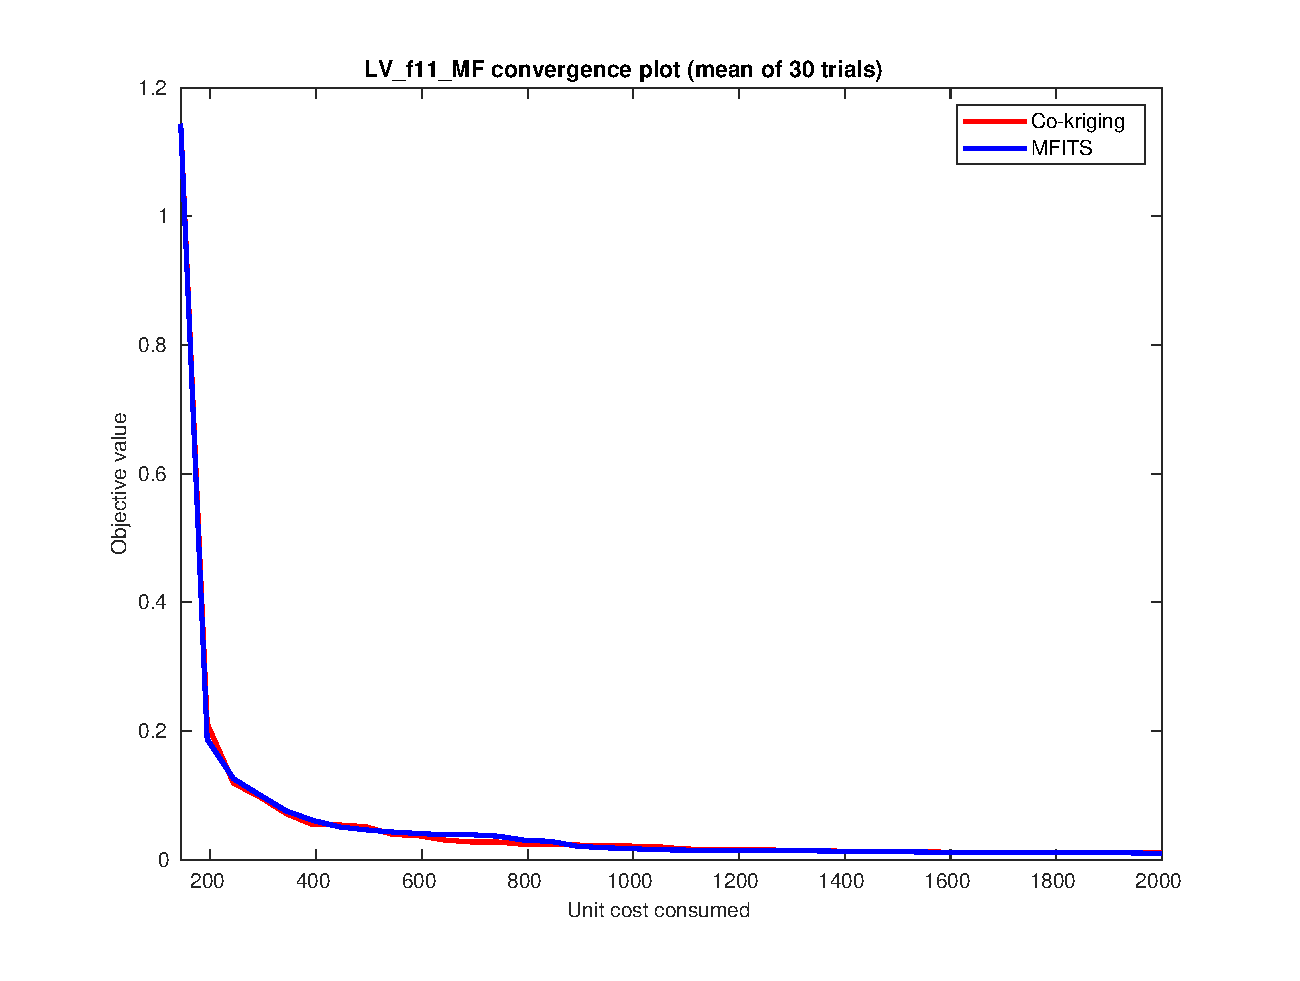
\includegraphics[width = 0.40\textwidth]{img/LV_f11_MF_conv_mean.eps} 
  \caption{Convergence plot for $f11$ function ($D=3$).\angus{will do a pgfplots version once finalised}} 
    \label{fig:f11-conv}
\end{figure}

\begin{figure}[h!]
  \centering
  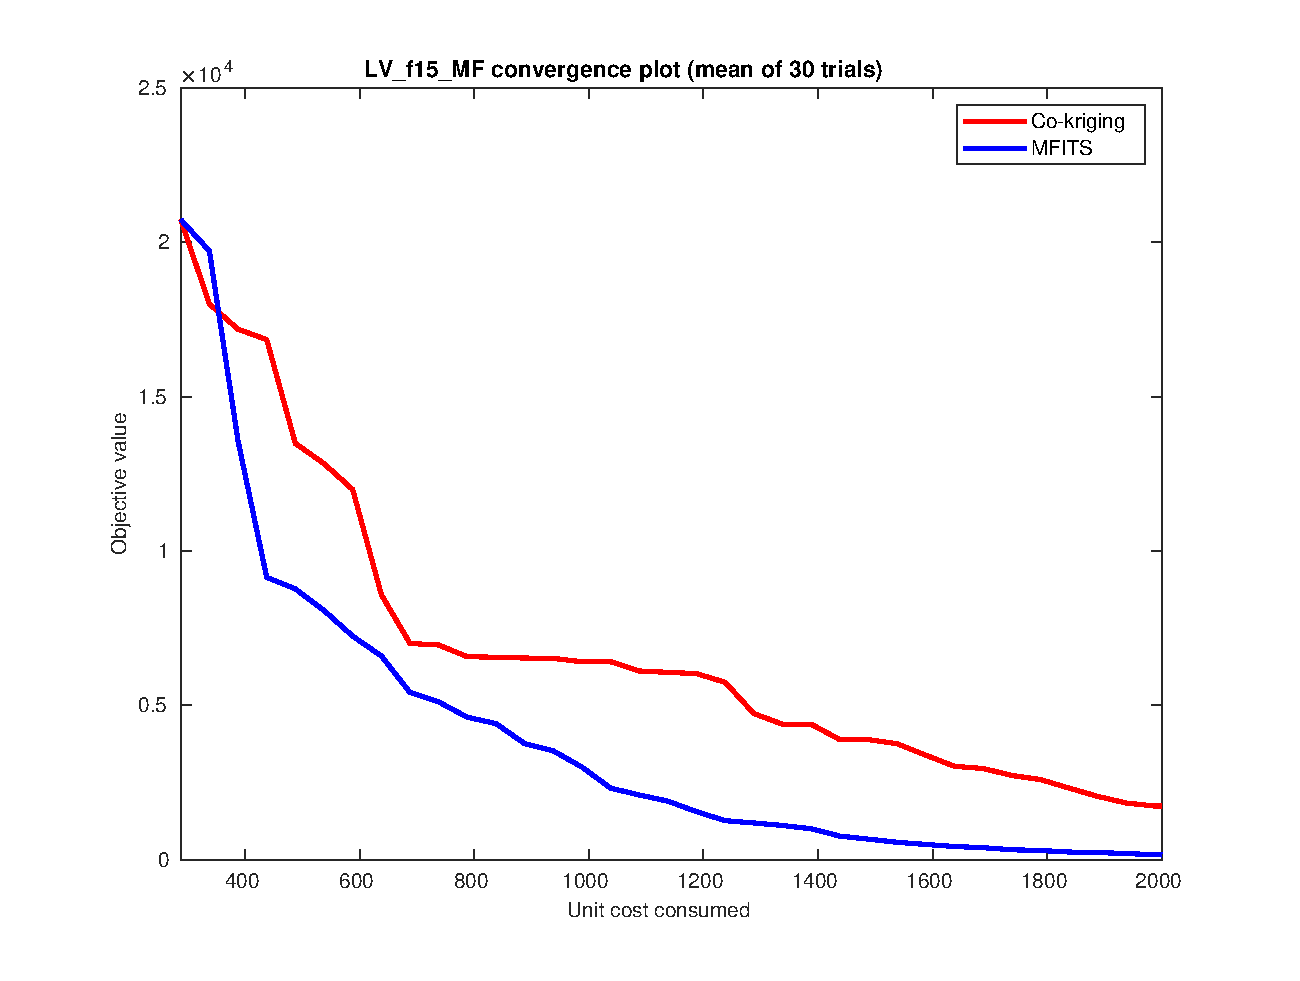
\includegraphics[width = 0.40\textwidth]{img/LV_f15_MF_conv_mean.eps} 
  \caption{Convergence plot for $f15$ function ($D=6$).\angus{will do a pgfplots version once finalised}} 
    \label{fig:f15-conv}
\end{figure}

\begin{figure}[h!]
  \centering
  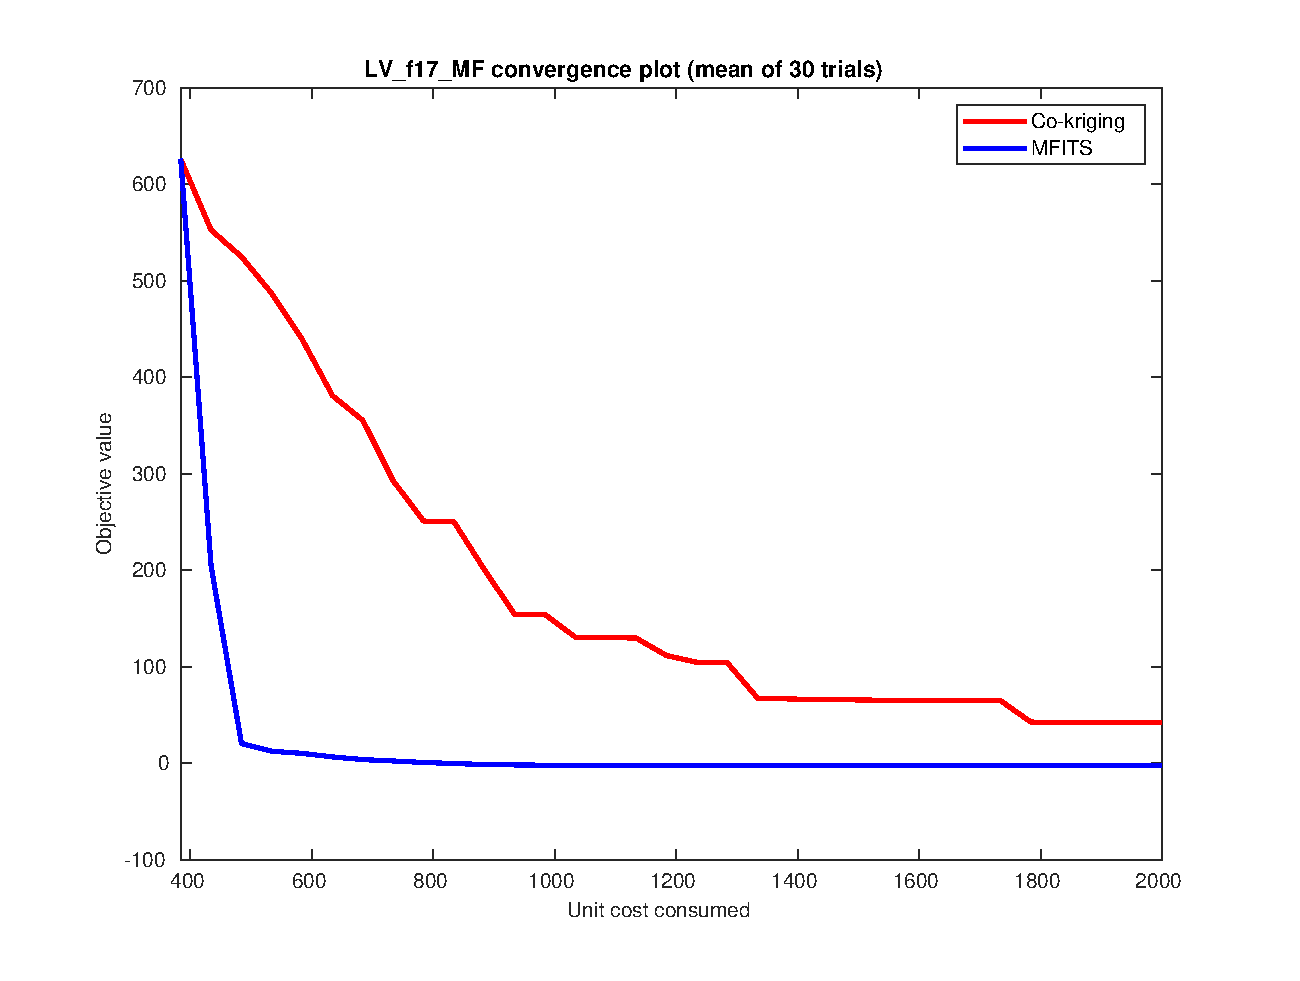
\includegraphics[width = 0.40\textwidth]{img/LV_f17_MF_conv_mean.eps} 
  \caption{Convergence plot for $f17$ function ($D=8$).\angus{will do a pgfplots version once finalised}} 
    \label{fig:f17-conv}
\end{figure}

\begin{table*}[h!]
\centering
\caption{Results \angus{some final tests running} on Griewank and Michalewicz test problems using Wang error functions 2 and 6 (indicated by subscript), comparing the base-line co-kriging algorithm to \AlgName{}. Given are the number of decision variables ($D$), the square of the Pearson correlation coefficient ($r^2$), the best objective obtained, the mean best objective over the full set of runs ($\mu$) and the corresponding standard deviation ($\sigma$).}\label{tab:results}
% \begin{adjustbox}{width=\columnwidth}
\begin{tabular}{lrrrrrrrr} \toprule
& & & \multicolumn{3}{c}{Co-kriging} & \multicolumn{3}{c}{\AlgName{}}\\
\cmidrule(lr){4-6} \cmidrule(lr){7-9}
Instance & $D$ & $r^2$ & \multicolumn{1}{c}{best}&\multicolumn{1}{c}{\(\mu\)} & \multicolumn{1}{c}{\(\sigma\)}&\multicolumn{1}{c}{best}& \multicolumn{1}{c}{\(\mu\)}&\multicolumn{1}{c}{\(\sigma\)}\\ \midrule
%
$Griewank_{2}$    & 3 & 0.73 &        0 &  0.0072 &  0.0137 &       0 &   0.0018 &  0.0083\\
                  & 5 & 0.54 &        0 &  0.0485 &  0.1055 &       0 &   0.0410 &  0.0674\\%
                  & 8 & 0.37 &        0 &  0.6538 &  0.3363 &       0 &   0.1864 &  0.2531\\
$Griewank_{6}$    & 3 & 0.74 &        0 &  0.0056 &  0.0114 &       0 &   0.0104 &  0.0130\\
                  & 5 & 0.76 &        0 &  0.0730 &  0.1145 &       0 &   0.0361 &  0.0778\\
                  & 8 & 0.76 &        0 &  0.4560 &  0.4238 &       0 &   0.2089 &  0.3539\\
\midrule  
$Michalewicz_{2}$ & 3 & 0.77 &  -2.7239 & -2.3582 &  0.2587 & -2.6716 &  -2.5305 &  0.1557\\
                  & 5 & 0.73 &  -3.5164 & -2.9470 &  0.2921 & -3.2890 &  -2.9953 &  0.3219\\%
\angus{still going}& 8 & 0.64 &  -4.3813 & -3.1214 &  0.5671 & -4.2150 &  -3.1352 &  0.7827\\
$Michalewicz_{6}$ & 3 & 0.76 &  -2.7194 & -2.2412 &  0.2978 & -2.6071 &  -2.3142 &  0.2411\\
\angus{still going}& 5 & 0.83 &  -4.1386 & -3.0140 &  0.3948 & -3.2785 &  -2.9104 &  0.2823\\
\angus{still going}& 8 & 0.86 &  -3.9978 & -3.1032 &  0.4929 & -3.2006 &  -3.1363 &  0.0909\\
%
\bottomrule
\end{tabular}
% \end{adjustbox}
\end{table*}

Notes for second dataset:
\begin{itemize}
\item when low dimensionality there is not much difference between the two (fig~\ref{fig:gw3-conv})
\item as with first dataset, at medium sized problems \AlgName{} finds slightly better solutions and converges a bit quicker (fig~\ref{fig:gw5-conv})
\item much bigger differences for the larger problem in both quality of solution and convergence rate (fig~\ref{fig:gw8-conv})
\end{itemize}

\begin{figure}[h!]
  \centering
  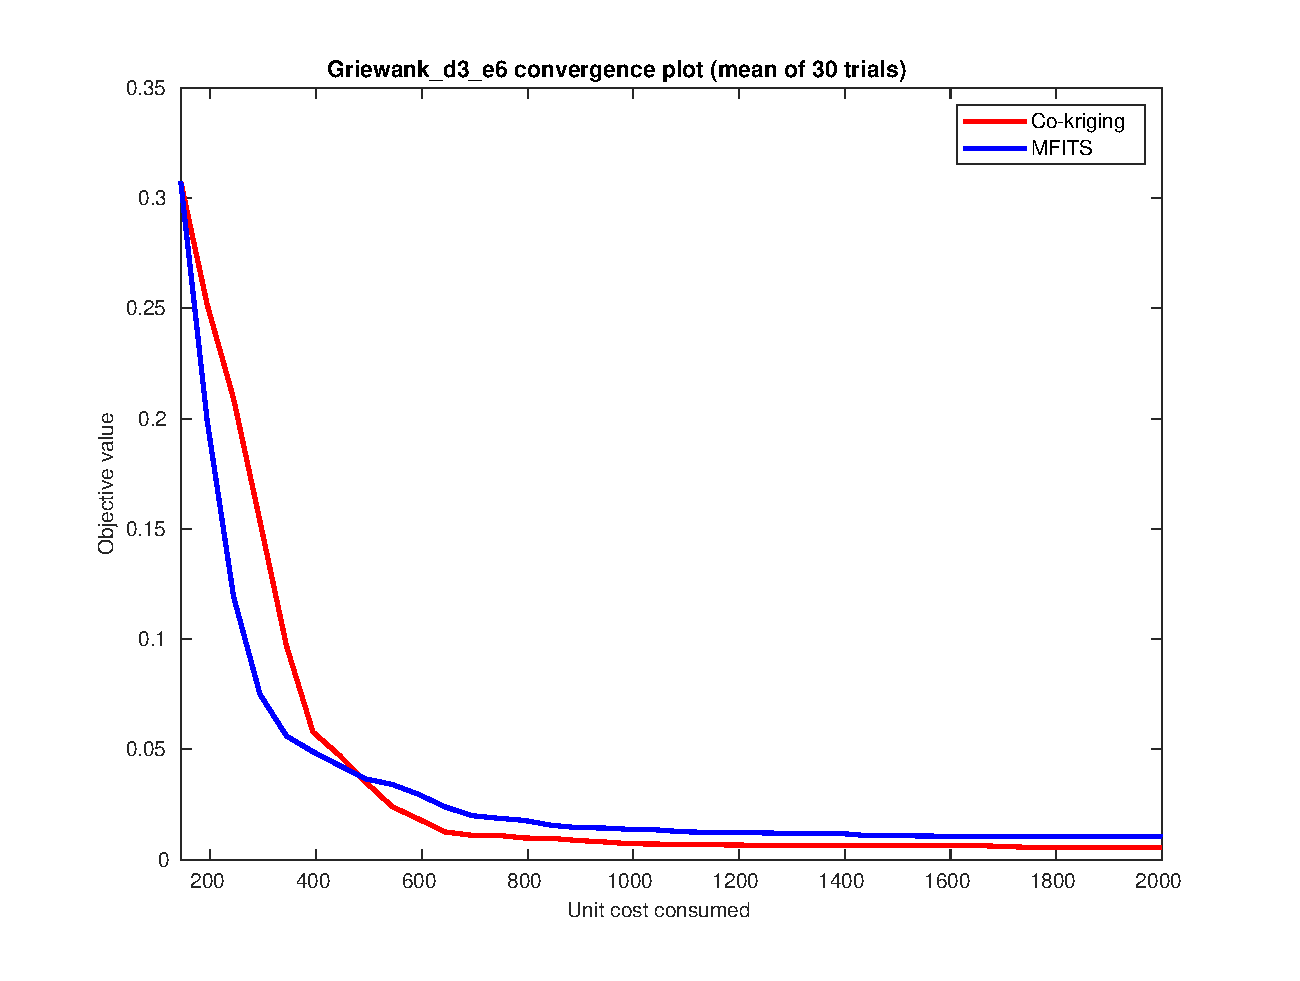
\includegraphics[width = 0.40\textwidth]{img/GW_d3_e6_conv_mean.eps} 
  \caption{Convergence plot for Griewank function with 3 decision variables and error function $e_6$.\angus{will do a pgfplots version once finalised}} 
    \label{fig:gw3-conv}
\end{figure}

\begin{figure}[h!]
  \centering
  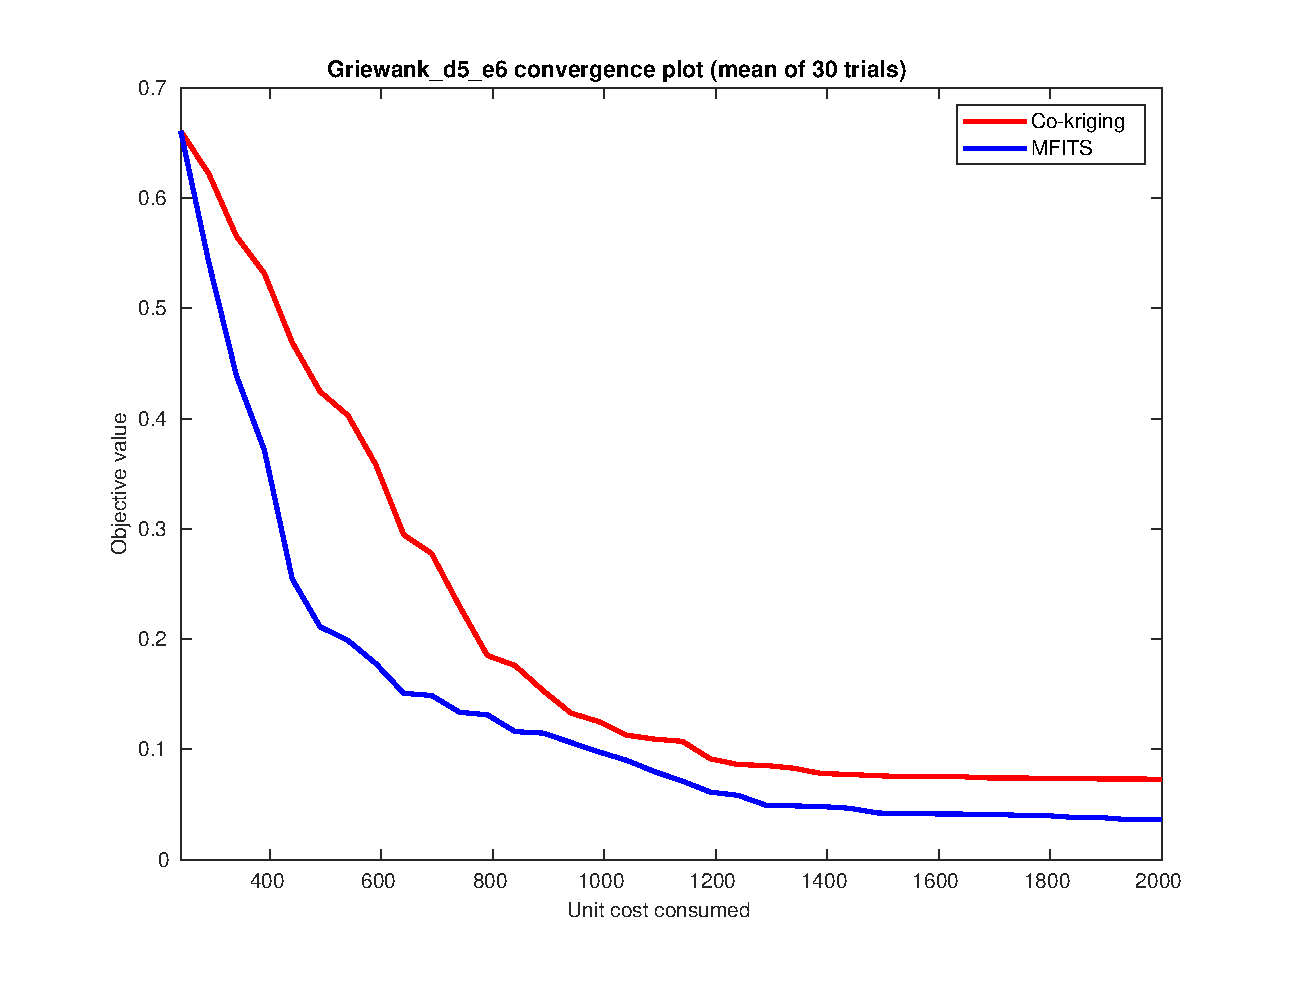
\includegraphics[width = 0.40\textwidth]{img/GW_d5_e6_conv_mean.eps} 
  \caption{Convergence plot for Griewank function with 5 decision variables and error function $e_6$.\angus{will do a pgfplots version once finalised}} 
    \label{fig:gw5-conv}
\end{figure}

\begin{figure}[h!]
  \centering
  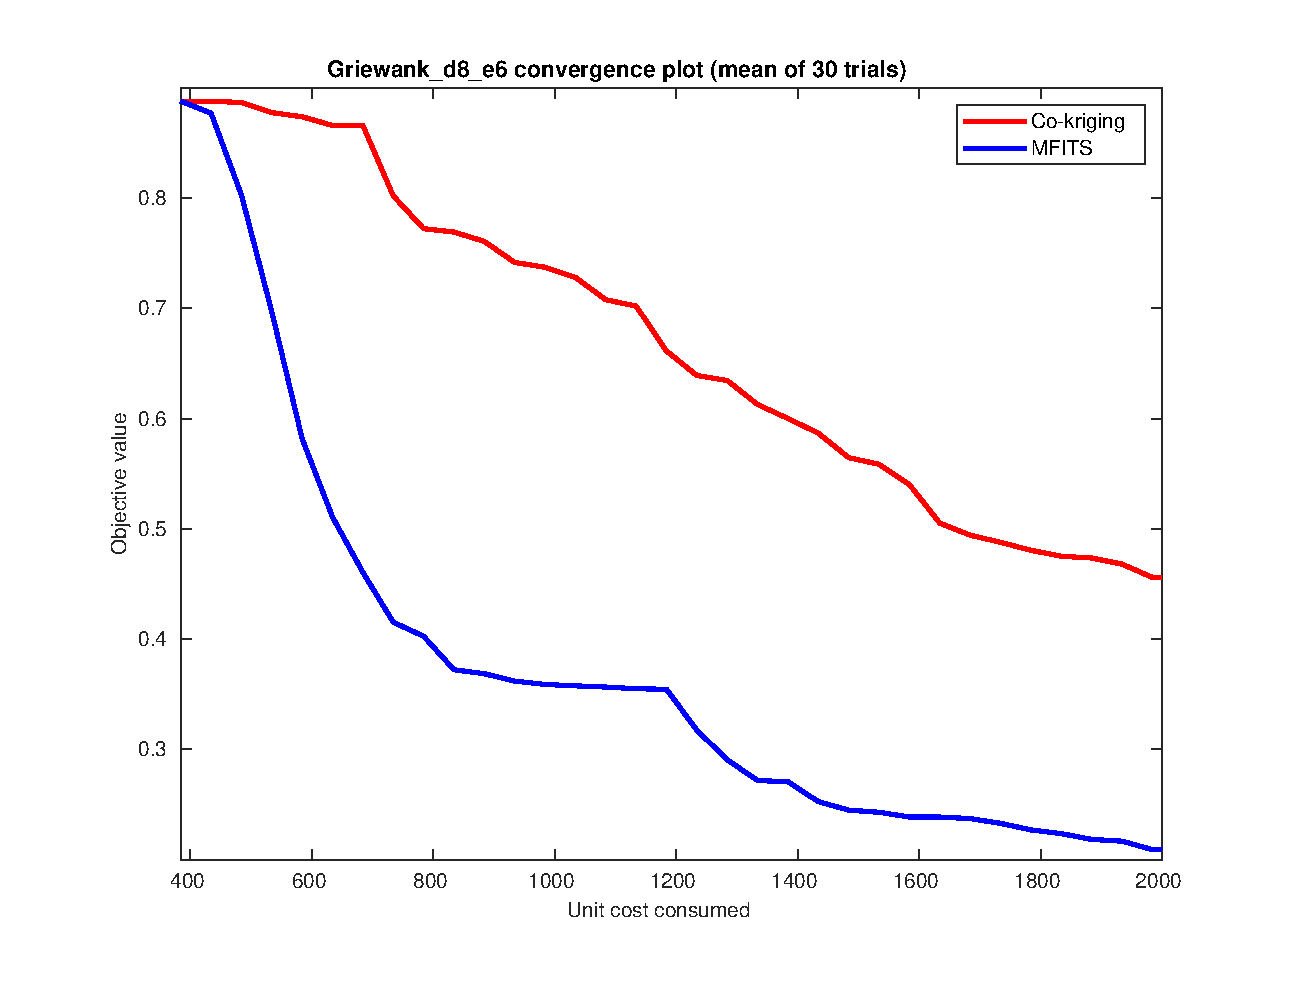
\includegraphics[width = 0.40\textwidth]{img/GW_d8_e6_conv_mean.eps} 
  \caption{Convergence plot for Griewank function with 8 decision variables and error function $e_6$.\angus{will do a pgfplots version once finalised}} 
    \label{fig:gw8-conv}
\end{figure}

General notes:
\begin{itemize}
\item first dataset shows that the results are consistent across a wide range of problems
\item second dataset allows for better comparison of the techniques across problem sizes
\item the results of both datasets agree with each other
\item in general, \AlgName{} will find better solutions than co-kriging as problem size increases
\item the real strength is in the covergence rate, which improves on co-kriging significantly as the size of the problem increases
\end{itemize}

\section{Conclusion and Future Work}\label{sec:conc}
\begin{itemize}
\item give conclusion
\item future work includes adding constraints
\end{itemize}


% \subsection{Subsection Heading Here}
% Subsection text here.

% % needed in second column of first page if using \IEEEpubid
% %\IEEEpubidadjcol

% \subsubsection{Subsubsection Heading Here}
% Subsubsection text here.


% % An example of a floating figure using the graphicx package.
% % Note that \label must occur AFTER (or within) \caption.
% % For figures, \caption should occur after the \includegraphics.
% % Note that IEEEtran v1.7 and later has special internal code that
% % is designed to preserve the operation of \label within \caption
% % even when the captionsoff option is in effect. However, because
% % of issues like this, it may be the safest practice to put all your
% % \label just after \caption rather than within \caption{}.
% %
% % Reminder: the "draftcls" or "draftclsnofoot", not "draft", class
% % option should be used if it is desired that the figures are to be
% % displayed while in draft mode.
% %
% %\begin{figure}[!t]
% %\centering
% %\includegraphics[width=2.5in]{myfigure}
% % where an .eps filename suffix will be assumed under latex, 
% % and a .pdf suffix will be assumed for pdflatex; or what has been declared
% % via \DeclareGraphicsExtensions.
% %\caption{Simulation results for the network.}
% %\label{fig_sim}
% %\end{figure}

% % Note that the IEEE typically puts floats only at the top, even when this
% % results in a large percentage of a column being occupied by floats.


% % An example of a double column floating figure using two subfigures.
% % (The subfig.sty package must be loaded for this to work.)
% % The subfigure \label commands are set within each subfloat command,
% % and the \label for the overall figure must come after \caption.
% % \hfil is used as a separator to get equal spacing.
% % Watch out that the combined width of all the subfigures on a 
% % line do not exceed the text width or a line break will occur.
% %
% %\begin{figure*}[!t]
% %\centering
% %\subfloat[Case I]{\includegraphics[width=2.5in]{box}%
% %\label{fig_first_case}}
% %\hfil
% %\subfloat[Case II]{\includegraphics[width=2.5in]{box}%
% %\label{fig_second_case}}
% %\caption{Simulation results for the network.}
% %\label{fig_sim}
% %\end{figure*}
% %
% % Note that often IEEE papers with subfigures do not employ subfigure
% % captions (using the optional argument to \subfloat[]), but instead will
% % reference/describe all of them (a), (b), etc., within the main caption.
% % Be aware that for subfig.sty to generate the (a), (b), etc., subfigure
% % labels, the optional argument to \subfloat must be present. If a
% % subcaption is not desired, just leave its contents blank,
% % e.g., \subfloat[].


% % An example of a floating table. Note that, for IEEE style tables, the
% % \caption command should come BEFORE the table and, given that table
% % captions serve much like titles, are usually capitalized except for words
% % such as a, an, and, as, at, but, by, for, in, nor, of, on, or, the, to
% % and up, which are usually not capitalized unless they are the first or
% % last word of the caption. Table text will default to \footnotesize as
% % the IEEE normally uses this smaller font for tables.
% % The \label must come after \caption as always.
% %
% %\begin{table}[!t]
% %% increase table row spacing, adjust to taste
% %\renewcommand{\arraystretch}{1.3}
% % if using array.sty, it might be a good idea to tweak the value of
% % \extrarowheight as needed to properly center the text within the cells
% %\caption{An Example of a Table}
% %\label{table_example}
% %\centering
% %% Some packages, such as MDW tools, offer better commands for making tables
% %% than the plain LaTeX2e tabular which is used here.
% %\begin{tabular}{|c||c|}
% %\hline
% %One & Two\\
% %\hline
% %Three & Four\\
% %\hline
% %\end{tabular}
% %\end{table}


% % Note that the IEEE does not put floats in the very first column
% % - or typically anywhere on the first page for that matter. Also,
% % in-text middle ("here") positioning is typically not used, but it
% % is allowed and encouraged for Computer Society conferences (but
% % not Computer Society journals). Most IEEE journals/conferences use
% % top floats exclusively. 
% % Note that, LaTeX2e, unlike IEEE journals/conferences, places
% % footnotes above bottom floats. This can be corrected via the
% % \fnbelowfloat command of the stfloats package.




% \section{Conclusion}
% The conclusion goes here.





% % if have a single appendix:
% %\appendix[Proof of the Zonklar Equations]
% % or
% %\appendix  % for no appendix heading
% % do not use \section anymore after \appendix, only \section*
% % is possibly needed

% % use appendices with more than one appendix
% % then use \section to start each appendix
% % you must declare a \section before using any
% % \subsection or using \label (\appendices by itself
% % starts a section numbered zero.)
% %


\appendices
\section{Function Equations}\label{app:testfuncs}
\begin{table*}[h!]
\centering
\caption{Test functions used for experiments in this paper. Given are the instance name, the function, the number of decision variables ($D$), the bounds ($B$) and the reference the test function is taken from.}\label{tab:funcs}
% \begin{adjustbox}{width=\columnwidth}
{%\scriptsize
\begin{tabular}{llrrr} \toprule
Instance & Function & $D$ & $B$ & Ref. \\ \midrule
%
$f10$         & $f_H(\V{x}) = 100\lr{\exp\lr{-\frac{2}{x_1^{1.75}}} + \exp\lr{-\frac{2}{x_2^{1.5}}} + \exp\lr{-\frac{2}{x_3^{1.25}}}}$ & $3$ & $[0,1]^D$ & \cite{lv2021multi}\\[0.3cm]
              & $f_L(\V{x}) = 100\lr{\exp\lr{-\frac{2}{x_1^{1.75}}} + \exp\lr{-\frac{2}{x_2^{1.5}}}}$\\
\midrule
$f11$         & $f_H(\V{x}) = 4\lr{x_1 - 2 + 8x_2 - 8x_2^2}^2 + \lr{3 - 4x_2}^2 + 16\sqrt{x_3 + 1}\lr{2x_3 - 1}^2$ & $3$ & $[0,1]^D$ & \cite{lv2021multi}\\[0.3cm]
              & $f_L(\V{x}) = 4\lr{x_1 - 2 + 8x_2 - 8x_2^2}^2 + \lr{3 - 4x_2}^2 + 5\sqrt{x_3 + 1}\lr{2x_3 - 1}^2$\\
\midrule
$f12$         & $f_H(\V{x}) = -\dsum{i=1}{m}\lr{\dsum{j=1}{4}(x_j - C_{ji})^2 + \beta_i}^{-1}$ & $4$ & $[0,10]^D$ & \cite{lv2021multi}\\[0.3cm]
              & $f_L(\V{x}) = -\dsum{i=1}{m}\lr{\dsum{j=1}{4}(x_j - C_{ji})^2 + 0.9\beta_i}^{-1}$\\[0.5cm]
              & $m = 10,\quad \beta = \frac{1}{10}(1,2,2,4,4,6,3,7,5,5)^T$\\[0.3cm]
              & $C = \begin{pmatrix}
                    4.0 & 1.0 & 8.0 & 6.0 & 3.0 & 2.0 & 5.0 & 8.0 & 6.0 & 7.0\\
                    4.0 & 1.0 & 8.0 & 6.0 & 7.0 & 9.0 & 3.0 & 1.0 & 2.0 & 3.6\\
                    4.0 & 1.0 & 8.0 & 6.0 & 3.0 & 2.0 & 5.0 & 8.0 & 6.0 & 7.0\\
                    4.0 & 1.0 & 8.0 & 6.0 & 7.0 & 9.0 & 3.0 & 1.0 & 2.0 & 3.6
                    \end{pmatrix}$\\
\midrule
$f13$         & $f_H(\V{x}) = (x_1 - 1)^2 + \dsum{i=2}{d}i\lr{2x_i^2 - x_{i-1}}^2$ & $4$ & $[-10,10]^D$ & \cite{lv2021multi}\\[0.3cm]
              & $f_L(\V{x}) = (x_1 - 1)^2 + x_2^4 + 4x_3^4 + 4x_4^4$\\
\midrule
$f14$         & $f_H(\V{x}) = \dsum{i=1}{5}\lr{0.3 + \sin\lr{\frac{16}{15}x_i - 1} + \sin\lr{\frac{16}{15}x_i - 1}^2}$ & $5$ & $[-1,1]^D$ & \cite{lv2021multi}\\[0.3cm]
              & $f_L(\V{x}) = \dsum{i=1}{5}\lr{0.3 + \sin\lr{\frac{13}{15}x_i - 1} + \sin\lr{\frac{13}{15}x_i - 1}^2}$\\
\midrule
$f15$         & $f_H(\V{x}) = \dsum{i=1}{5}\lr{100\lr{x_{i+1} - x_i^2}^2 + \lr{x_i - 1}^2}$ & $6$ & $[0,1]^D$ & \cite{lv2021multi}\\[0.3cm]
              & $f_L(\V{x}) = \dsum{i=1}{5}\lr{100\lr{x_{i+1} - x_i^2}^2 + 4\lr{x_i - 1}^4}$\\
\midrule
$f16$         & $f_H(\V{x}) = \dsum{i=1}{2}\lrsq{\begin{matrix}\lr{4x_{4i-3} - 10x_{4i-2}}^2 + 5\lr{x_{4i-1} - x_{4i}}^2 +\\\lr{x_{4i-2} - 2x_{4i-1}}^4 + 10\lr{x_{4i-3} - x_{4i}}^2\end{matrix}}$ & $8$ & $[-4,5]^D$ & \cite{lv2021multi}\\[0.3cm]
              & $f_L(\V{x}) = \dsum{i=1}{2}\lrsq{\begin{matrix}\lr{4x_{4i-3} - 10x_{4i-2}}^2 + 5\lr{x_{4i-1} - x_{4i}}^2 +\\\lr{x_{4i-2} - 2x_{4i-1}}^4 + 4\lr{x_{4i-3} - x_{4i}}^2\end{matrix}}$\\
\midrule
$f17$         & $f_H(\V{x}) = \dsum{i=1}{8}\lr{x_i^4 - 16x_i^2 + 5x_i}$ & $8$ & $[-5,5]^D$ & \cite{lv2021multi}\\[0.3cm]
              & $f_L(\V{x}) = \dsum{i=1}{8}\lr{0.8x_i^4 - 16x_i^2 + 5x_i}$\\
\midrule
$Griewank$    & $f_H(\V{x}) = \displaystyle\sum^D_{i = 1} \frac{x_i^2}{4000} - \prod^D_{i = 1}\cos{\left(\frac{x_i}{\sqrt{i}}\right)}+1$ & $\{3,5,8\}$ & $[-5,5]^D$ &\\
\midrule  
$Michalewicz$ & $f_H(\V{x}) = \displaystyle\sum^D_{i = 1} \sin{\left(x_i\right)}\sin^{2m}{\left(\frac{ix_i^2}{\pi}\right)},\quad m = 10$ & $\{3,5,8\}$ & $[0,\pi]^D$&\\
%
\bottomrule
\end{tabular}
}
% \end{adjustbox}
\end{table*}

\begin{table*}[h!]
\centering
\caption{Error functions used, as defined in Wang~et~al.~\cite{wang2017generic}. Function $e_2$ models resolution errors and $e_6$ models stochastic errors. Here, $\phi \in [0,10000]$ determines the fidelity level and $D$ is the number of decision variables.}\label{tab:errfuncs}
% \begin{adjustbox}{width=\columnwidth}
{%\scriptsize
\begin{tabular}{ll} \toprule
Name & Function \\ \midrule
%
$e_2$         & $e_2(\V{x},\phi) = \dsum{i=1}{D}a(\phi)\cos{\left(w(\phi)x_i+b(\phi)+\pi\right)}$\\[0.3cm]
              & where, $a(\phi) = \theta(\phi),\ w(\phi) = 10\pi\theta(\phi),\ b(\phi) = 0.5\pi\theta(\phi),\ \theta(\phi) = e^{-0.00025\phi}$\\
\midrule
$e_6$         & $e_6 = \mathcal{N}\left(\mu(\V{x},\phi),\sigma(\phi)\right)$ \\[0.3cm]
              & where, $\mu^2(\phi) = 0,\ \sigma(\phi) = 0.1\vartheta(\phi),\ \vartheta(\phi) = e^{-0.0005\phi}$\\
\bottomrule
\end{tabular}
}
% \end{adjustbox}
\end{table*}


% % you can choose not to have a title for an appendix
% % if you want by leaving the argument blank
% \section{}
% Appendix two text goes here.


% % use section* for acknowledgment
% \section*{Acknowledgment}


% The authors would like to thank...


% % Can use something like this to put references on a page
% % by themselves when using endfloat and the captionsoff option.
% \ifCLASSOPTIONcaptionsoff
%   \newpage
% \fi



% % trigger a \newpage just before the given reference
% % number - used to balance the columns on the last page
% % adjust value as needed - may need to be readjusted if
% % the document is modified later
% %\IEEEtriggeratref{8}
% % The "triggered" command can be changed if desired:
% %\IEEEtriggercmd{\enlargethispage{-5in}}

% % references section

% % can use a bibliography generated by BibTeX as a .bbl file
% % BibTeX documentation can be easily obtained at:
% % http://mirror.ctan.org/biblio/bibtex/contrib/doc/
% % The IEEEtran BibTeX style support page is at:
% % http://www.michaelshell.org/tex/ieeetran/bibtex/
\bibliographystyle{IEEEtran}
% argument is your BibTeX string definitions and bibliography database(s)
\bibliography{refs.bib}
% %
% % <OR> manually copy in the resultant .bbl file
% % set second argument of \begin to the number of references
% % (used to reserve space for the reference number labels box)
% \begin{thebibliography}{1}

% \bibitem{IEEEhowto:kopka}
% H.~Kopka and P.~W. Daly, \emph{A Guide to \LaTeX}, 3rd~ed.\hskip 1em plus
%   0.5em minus 0.4em\relax Harlow, England: Addison-Wesley, 1999.

% \end{thebibliography}

% % biography section
% % 
% % If you have an EPS/PDF photo (graphicx package needed) extra braces are
% % needed around the contents of the optional argument to biography to prevent
% % the LaTeX parser from getting confused when it sees the complicated
% % \includegraphics command within an optional argument. (You could create
% % your own custom macro containing the \includegraphics command to make things
% % simpler here.)
% %\begin{IEEEbiography}[{\includegraphics[width=1in,height=1.25in,clip,keepaspectratio]{mshell}}]{Michael Shell}
% % or if you just want to reserve a space for a photo:

% \begin{IEEEbiography}{Michael Shell}
% Biography text here.
% \end{IEEEbiography}

% % if you will not have a photo at all:
% \begin{IEEEbiographynophoto}{John Doe}
% Biography text here.
% \end{IEEEbiographynophoto}

% % insert where needed to balance the two columns on the last page with
% % biographies
% %\newpage

% \begin{IEEEbiographynophoto}{Jane Doe}
% Biography text here.
% \end{IEEEbiographynophoto}

% % You can push biographies down or up by placing
% % a \vfill before or after them. The appropriate
% % use of \vfill depends on what kind of text is
% % on the last page and whether or not the columns
% % are being equalized.

% %\vfill

% % Can be used to pull up biographies so that the bottom of the last one
% % is flush with the other column.
% %\enlargethispage{-5in}



% that's all folks
\end{document}


